% Alternativas de Solución
% Este archivo se incluye desde main.tex con \input.
\section{Alternativas de Solución}
\subsection{Introducción del Capítulo}
Una vez definida la metodología, en este capítulo se presentan las distintas alternativas de arquitectura y funcionalidades que se evaluaron para construir la solución. Cada alternativa tiene un nivel de complejidad distinto. La diferencia principal está en cómo se obtienen los datos cardiovasculares, que es la parte más variable desde el punto de vista técnico, pero también cambian el registro de nutrición, el uso de inteligencia artificial y el nivel de detalle del cruce de datos.
\\\\
Las tres alternativas comparten la misma base tecnológica y el mismo motor de cruce de datos, que funciona ordenando los eventos en el tiempo. Lo que cambia entre ellas es la cantidad y la calidad de los datos que recibe ese motor, y eso influye directamente en qué tan precisas son sus estimaciones de fatiga cruzada.
\subsection{Descripción de Alternativas}
\subsubsection{Base Tecnológica Común}

Sea cual sea la alternativa elegida, la solución se construirá con las siguientes tecnologías:

\begin{itemize}
    \item \textbf{Frontend Móvil:} Flutter (Dart), un framework multiplataforma que permite crear aplicaciones para Android e iOS con un solo código, lo que reduce el tiempo de desarrollo y mantenimiento.
    \item \textbf{Backend / API:} NestJS (Node.js con TypeScript), un framework para construir aplicaciones del lado del servidor. Su estructura por módulos facilita que el sistema crezca y que cada parte (nutrición, fuerza, cardio y analítica) quede separada.
    \newpage
    \item \textbf{Base de Datos:} MongoDB, una base de datos NoSQL orientada a documentos. Cada registro se guarda como un documento en formato BSON, sin necesidad de una estructura fija. Las sesiones de entrenamiento, las comidas y los datos de los dispositivos se guardan como documentos que se pueden consultar con índices aunque su estructura cambie (por ejemplo, una sesión de fuerza con 4 ejercicios y otra con 7).
    \item \textbf{Almacenamiento de Imágenes y Archivos:} Amazon S3, un servicio de almacenamiento de objetos, junto con Amazon CloudFront, una red de distribución de contenido (CDN) que guarda copias de las imágenes en servidores cercanos a los usuarios para que carguen rápido. Las fotos no se guardan dentro de MongoDB, porque harían crecer mucho la base de datos y sus respaldos. En la base de datos solo queda la dirección de cada archivo.
\end{itemize}

\textbf{Motor de Cruce de Datos Basado en Timestamps}

Lo que más diferencia a esta plataforma es que cruza los datos de fuerza, resistencia y nutrición para estimar la fatiga cruzada. El motor funciona ordenando todo en el tiempo. Cada evento registrado (una comida, una sesión de fuerza, una sesión de cardio o un reporte de sensaciones) se guarda con su fecha y hora exacta (timestamp). A partir de esa información, el motor calcula lo siguiente:

\begin{enumerate}
    \item \textbf{Ventanas de recuperación:} El tiempo que pasa entre el fin de una sesión de fuerza y el inicio de la siguiente sesión de cardio, y al revés. Compara ese tiempo con lo que recomienda la literatura (al menos 6 a 8 horas entre sesiones de distinto tipo) para avisar cuando hay riesgo de interferencia.
    \item \textbf{Horario de las comidas:} Revisa si las comidas se hicieron en los momentos recomendados respecto al entrenamiento. Por ejemplo, carbohidratos 2 a 3 horas antes del cardio, proteínas dentro de las 2 horas posteriores a la fuerza, o si se comió en el momento adecuado durante una ruta larga.
    \item \textbf{Fatiga acumulada semanal:} Suma el volumen de entrenamiento de los últimos 7 días. En fuerza se calcula como $\sum(\text{series} \times \text{repeticiones} \times \text{peso})$. En cardio, la medida depende de la alternativa, y va desde distancia $\times$ RPE en la más básica hasta una carga basada en zonas cardíacas y potencia en las más avanzadas.
    \item \textbf{Detección de interferencia:} Si en días seguidos hay secuencias de fuerza $\rightarrow$ cardio (o al revés) con poca recuperación entre ellas, el sistema muestra una alerta y sugiere reorganizar el calendario.
\end{enumerate}

La lógica del motor es \textbf{la misma} en las tres alternativas. Lo que cambia es la \textbf{calidad y el nivel de detalle de los datos que recibe}. Mientras más información tenga (frecuencia cardíaca, potencia, cadencia), más precisas serán sus estimaciones.

\textbf{Almacenamiento de Imágenes}

Las tres alternativas guardan fotos, aunque en cantidades muy distintas. La Alternativa 1 solo guarda la foto de perfil, la Alternativa 2 agrega una foto por receta compartida y la Alternativa 3 permite hasta 4 fotos por publicación en la red social. Para que las fotos no encarezcan ni hagan más lenta la aplicación, las tres siguen el mismo esquema:

\begin{enumerate}
    \item El teléfono reduce la foto a un máximo de 1080 píxeles por lado y la comprime, dejándola en unos 300 KB. También crea una miniatura de unos 40 KB para mostrarla en el muro y le borra los datos de ubicación (EXIF).
    \item La aplicación le pide al backend un permiso de subida que dura pocos minutos (URL prefirmada). Con ese permiso, el teléfono sube la foto directamente a Amazon S3, sin pasar por el servidor de NestJS, que así no tiene que recibir archivos pesados.
    \item El backend guarda en MongoDB solo la dirección de la foto, dentro del documento al que pertenece (por ejemplo, la publicación o el perfil).
    \item Para mostrar las fotos, la aplicación las pide a Amazon CloudFront, que las mantiene en caché. El bucket de S3 es privado y solo CloudFront puede leerlo.
    \item Una regla automática del bucket borra las fotos que se subieron pero nunca se publicaron, y las de publicaciones o cuentas eliminadas.
\end{enumerate}

Las fotos que se sacan solo para registrar una comida con IA no pasan por S3. El backend las envía al servicio de IA y las descarta después del análisis, salvo que el usuario decida publicarlas.
\\\\
También se evaluaron otras opciones. Guardar las fotos dentro de MongoDB (con GridFS) haría crecer la base de datos administrada, que cobra más por cada GB que S3, y volvería más lentos los respaldos. Servicios como Firebase Storage o Cloudflare R2 también servirían, pero sumarían otro proveedor. Como el resto de la infraestructura ya está en AWS y el nivel gratuito de CloudFront cubre la entrega de las fotos, se eligió S3 con CloudFront. El costo de este esquema se calcula en la factibilidad económica (Tabla \ref{tab:costo_imagenes}).

\subsubsection{Alternativa 1: Solución Minimalista (MVP Lean)}

\textbf{Descripción General}

Esta alternativa es la versión más simple que todavía permite abordar el problema del entrenamiento concurrente. Busca reducir el costo y el tiempo de desarrollo, a cambio de tener menos automatización y datos menos precisos. Está pensada para usuarios que no tienen wearables y que están dispuestos a registrar su actividad a mano.
\\\\
\textbf{Módulo de Nutrición}

Las comidas se registran solo con formularios. El usuario elige los ingredientes desde una base de datos alimentada por una API gratuita de alimentos (como OpenFoodFacts) e ingresa las cantidades. El sistema calcula automáticamente los macronutrientes y las calorías de cada comida. No se usa inteligencia artificial para estimar la comida a partir de fotos ni de texto libre.
\\\\
\textbf{Módulo de Fuerza}

El usuario crea rutinas base (plantillas de ejercicios) y registra cada sesión con un formulario, eligiendo el ejercicio e ingresando series, repeticiones y peso. Incluye un campo de texto libre para anotar las sensaciones de cada ejercicio. No se incluye registro por lenguaje natural.
\newpage
\textbf{Módulo de Cardio}

El registro de cardio usa solo el GPS del teléfono y la percepción del esfuerzo (RPE). La aplicación graba la ruta, la velocidad, la distancia y el tiempo con la ubicación del teléfono. Al terminar la sesión, el usuario indica su RPE en una escala de 1 a 10 y puede agregar notas. No hay integración con wearables, Health Connect, Apple Health ni archivos \texttt{.fit}.
\\\\
\textbf{Motor de Cruce de Datos}

En este caso el motor de cruce trabaja con pocos datos. La fatiga del cardio se estima a partir de la distancia, el tiempo y el RPE. Como no hay datos de frecuencia cardíaca, no se pueden calcular las zonas de entrenamiento ni el gasto real de calorías, así que las estimaciones de fatiga cruzada son aproximaciones basadas en lo que el usuario declara.
\\\\
\textbf{Módulo Social}

Incluye una comunidad básica donde los usuarios pueden compartir rutas, rutinas de fuerza y recetas. No incluye el ajuste automático de porciones. Las publicaciones no llevan fotos, así que las únicas imágenes que guarda esta alternativa son las fotos de perfil.
\\\\
\textbf{Arquitectura de la Solución}

La arquitectura de esta alternativa es monolítica y sencilla. La aplicación móvil (Flutter) se comunica con una API REST hecha en NestJS, que contiene toda la lógica de negocio y guarda los datos en MongoDB. Las fotos de perfil se suben directamente desde el teléfono a Amazon S3 y se muestran a través de CloudFront.

\vspace{0.5cm}
\begin{center}
\setstretch{1}
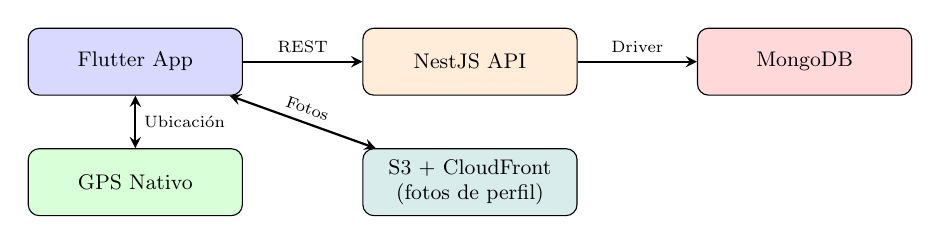
\begin{tikzpicture}[
    node distance=1.8cm,
    box/.style={draw, rectangle, rounded corners, minimum width=3.2cm, minimum height=1cm, fill=#1, text centered, font=\small},
    arrow/.style={->, thick, >=stealth},
    scale=0.85, transform shape
]
    % Frontend
    \node (app) [box=blue!15] {Flutter App};
    \node (gps) [box=green!15, below of=app] {GPS Nativo};

    % Backend
    \node (api) [box=orange!15, right of=app, node distance=5cm] {NestJS API};

    % Database
    \node (db) [box=red!15, right of=api, node distance=5cm] {MongoDB};

    % Arrows
    \draw[arrow] (app) -- node[above, font=\scriptsize] {REST} (api);
    \draw[arrow] (api) -- node[above, font=\scriptsize] {Driver} (db);
    \draw[arrow, <->] (app) -- node[right, font=\scriptsize] {Ubicación} (gps);

    % Fotos
    \node (s3) [box=teal!15, below of=api] {\shortstack{S3 + CloudFront\\(fotos de perfil)}};
    \draw[arrow, <->] (app) -- node[above, sloped, font=\scriptsize] {Fotos} (s3);

\end{tikzpicture}
\captionof{figure}{Arquitectura de la Alternativa 1: Solución Minimalista.}
\end{center}
\vspace{0.5cm}
\newpage
\textbf{Estimación de Costos}

La siguiente tabla resume los costos de esta alternativa. El costo de desarrollo viene del análisis por ciclo de vida (Tabla \ref{tab:ciclovida_alt1}), y los demás valores son los mismos que se usan en su flujo de caja dentro de la factibilidad económica.

\begin{table}[h!]
    \centering
    \renewcommand{\arraystretch}{1.4}
    \begin{tabular}{|m{4cm}|m{5.5cm}|r|}
        \hline
        \rowcolor[HTML]{EFEFEF}
        \textbf{Ítem} & \textbf{Detalle} & \textbf{Costo (CLP)} \\ \hline
        \multicolumn{3}{|l|}{\cellcolor[HTML]{E3F2FD}\textbf{Inversión inicial (Año 0)}} \\ \hline
        Desarrollo de software & 260 horas de trabajo según el ciclo de vida & \$8.545.627 \\ \hline
        Publicación en tiendas & Google Play y Apple Developer & \$120.602 \\ \hline
        \rowcolor[HTML]{E8F5E9}
        \textbf{Total inversión inicial} & & \textbf{\$8.666.229} \\ \hline
        \multicolumn{3}{|l|}{\cellcolor[HTML]{FFF3E0}\textbf{Costos operativos anuales (Años 1 a 4)}} \\ \hline
        Infraestructura Cloud & AWS (Fargate, ALB, IP públicas y CloudWatch) y MongoDB Atlas M10 (Tabla \ref{tab:costo_infra}) & \$1.879.063 \\ \hline
        Imágenes & S3 y CloudFront para las fotos de perfil (Tabla \ref{tab:costo_imagenes}) & \$11.671 \\ \hline
        APIs de IA & No utiliza IA & No aplica \\ \hline
        Mantenimiento & 10\% del costo de desarrollo & \$854.563 \\ \hline
        Suscripción Apple & Renovación anual del Apple Developer Program & \$96.287 \\ \hline
        \rowcolor[HTML]{FFF3E0}
        \textbf{Total operativo anual} & & \textbf{\$2.841.584} \\ \hline
    \end{tabular}
    \caption{Estimación de costos de la Alternativa 1: Solución Minimalista.}
    \label{tab:costos_alt1}
\end{table}

\newpage
\subsubsection{Alternativa 2: Solución Integrada con Brokers del Sistema Operativo}

\textbf{Descripción General}

Esta alternativa sigue lo que hoy hace la mayoría de las aplicaciones deportivas. Deja que los wearables del usuario registren los datos más pesados y los lee de forma automática desde los concentradores del sistema operativo, que son \textbf{Health Connect} en Android y \textbf{Apple Health (HealthKit)} en iOS. Además, usa inteligencia artificial para que registrar comidas y rutinas de fuerza sea más rápido.
\\\\
\textbf{Módulo de Nutrición}

Las comidas se pueden registrar de dos formas con ayuda de inteligencia artificial:
\begin{itemize}
    \item \textbf{Procesamiento de Lenguaje Natural (PLN):} El usuario describe su comida con sus propias palabras (por ejemplo, ``desayuné 3 huevos con avena y yogurt'') y el sistema separa los ingredientes y estima los macronutrientes.
    \item \textbf{Visión Artificial:} El usuario saca una foto a su plato y un modelo estima qué alimentos hay y en qué cantidad. Después, el usuario puede corregir el resultado.
\end{itemize}
Ambas funciones usan una API de inteligencia artificial en la nube (Gemini, con sus modelos Flash). La base de datos de alimentos se mantiene para validar y corregir los resultados.
\\\\
\textbf{Módulo de Fuerza}

Además del formulario, se agrega el registro por lenguaje natural. El usuario puede dictar o escribir su rutina (por ejemplo, ``hice 3 series de 10 sentadillas con 80 kilos'') y el sistema identifica el ejercicio, las series, las repeticiones y el peso, y los guarda en la base de datos. También se mantiene el registro de sensaciones de cada ejercicio.
\newpage
\textbf{Módulo de Cardio}

El sistema lee automáticamente los datos que reúnen Health Connect (Android) y Apple Health (iOS). Cuando el usuario termina una sesión de cardio registrada con un wearable compatible (Garmin, Polar, Apple Watch, Samsung Galaxy Watch, entre otros), los datos se sincronizan con el concentrador del teléfono y la aplicación los importa en segundo plano. Los datos disponibles a través de estos concentradores son:

\begin{itemize}
    \item Frecuencia cardíaca promedio y máxima de la sesión.
    \item Calorías activas estimadas por el dispositivo.
    \item Distancia recorrida y duración.
    \item Ruta GPS (cuando el wearable la registra).
    \item Zonas de ritmo cardíaco (calculadas por la aplicación a partir de la FC importada).
\end{itemize}

Además, se mantiene el GPS del teléfono como respaldo para usuarios sin wearable, junto con el RPE.
\\\\
\textbf{Motor de Cruce de Datos}

Al contar con la frecuencia cardíaca y las calorías activas reales, el motor de cruce es más preciso. Puede calcular las zonas de entrenamiento (Zona 1 a Zona 5) y separar el gasto calórico según el tipo de esfuerzo. Con eso, el módulo de nutrición puede ajustar los macronutrientes según la fuente de energía que más se usó (carbohidratos en zonas altas y grasas en zonas bajas). Las estimaciones de fatiga cruzada también mejoran, porque consideran la carga interna (el esfuerzo del corazón) y no solo la carga externa (volumen y distancia).
\\\\
\textbf{Módulo Social}

Incluye la comunidad para compartir rutas, rutinas y recetas, y agrega el ajuste automático de porciones. El sistema toma una receta de la comunidad y ajusta las cantidades de cada ingrediente para cubrir los macronutrientes que el usuario necesita según el desgaste del día. Cada receta compartida puede llevar una foto del plato, además de la foto de perfil de cada usuario.
\newpage
\textbf{Arquitectura de la Solución}

La arquitectura agrega la conexión con los SDKs de Health Connect y HealthKit, además de un servicio de inteligencia artificial en la nube para el procesamiento de lenguaje natural y la visión artificial. Las fotos de perfil y de las recetas se guardan en Amazon S3 y se muestran a través de CloudFront.

\vspace{0.5cm}
\begin{center}
\setstretch{1}
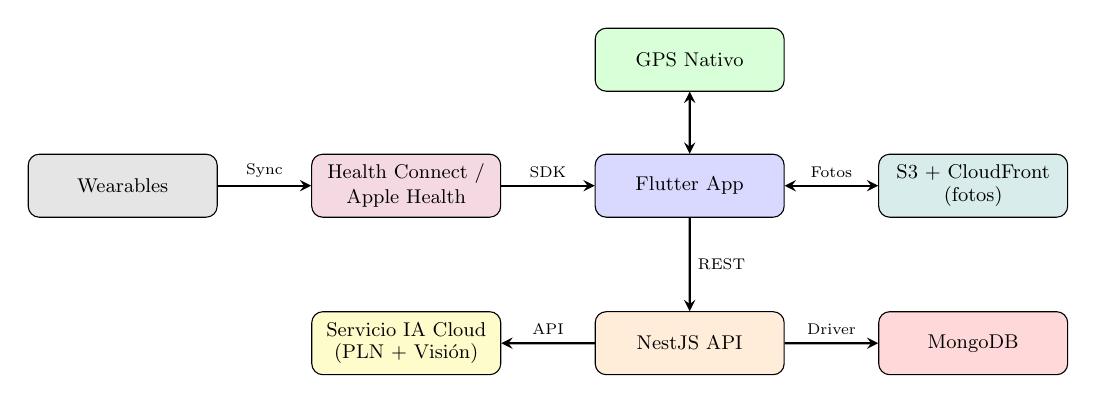
\begin{tikzpicture}[
    node distance=2cm,
    box/.style={draw, rectangle, rounded corners, minimum width=3cm, minimum height=1cm, fill=#1, text centered, font=\small},
    arrow/.style={->, thick, >=stealth},
    darrow/.style={<->, thick, >=stealth},
    scale=0.8, transform shape
]
    % External devices
    \node (wear) [box=gray!20] {Wearables};
    \node (hc) [box=purple!15, right of=wear, node distance=4.5cm] {\shortstack{Health Connect /\\Apple Health}};

    % Frontend
    \node (app) [box=blue!15, right of=hc, node distance=4.5cm] {Flutter App};

    % Backend
    \node (api) [box=orange!15, below of=app, node distance=2.5cm] {NestJS API};

    % AI Service
    \node (ai) [box=yellow!20, left of=api, node distance=4.5cm] {\shortstack{Servicio IA Cloud\\(PLN + Visión)}};

    % Database
    \node (db) [box=red!15, right of=api, node distance=4.5cm] {MongoDB};

    % GPS
    \node (gps) [box=green!15, above of=app, node distance=2cm] {GPS Nativo};

    % Arrows
    \draw[arrow] (wear) -- node[above, font=\scriptsize] {Sync} (hc);
    \draw[arrow] (hc) -- node[above, font=\scriptsize] {SDK} (app);
    \draw[arrow] (app) -- node[right, font=\scriptsize] {REST} (api);
    \draw[arrow] (api) -- node[above, font=\scriptsize] {Driver} (db);
    \draw[arrow] (api) -- node[above, font=\scriptsize] {API} (ai);
    \draw[darrow] (gps) -- node[right, font=\scriptsize] {} (app);

    % Fotos
    \node (s3) [box=teal!15, right of=app, node distance=4.5cm] {\shortstack{S3 + CloudFront\\(fotos)}};
    \draw[darrow] (app) -- node[above, font=\scriptsize] {Fotos} (s3);

\end{tikzpicture}
\captionof{figure}{Arquitectura de la Alternativa 2: Solución Integrada con Brokers del SO.}
\end{center}
\vspace{0.5cm}
\newpage
\textbf{Estimación de Costos}

La siguiente tabla resume los costos de esta alternativa. El costo de desarrollo viene del análisis por ciclo de vida (Tabla \ref{tab:ciclovida_alt2}), y los demás valores son los mismos que se usan en su flujo de caja dentro de la factibilidad económica.

\begin{table}[h!]
    \centering
    \renewcommand{\arraystretch}{1.4}
    \begin{tabular}{|m{4cm}|m{5.5cm}|r|}
        \hline
        \rowcolor[HTML]{EFEFEF}
        \textbf{Ítem} & \textbf{Detalle} & \textbf{Costo (CLP)} \\ \hline
        \multicolumn{3}{|l|}{\cellcolor[HTML]{E3F2FD}\textbf{Inversión inicial (Año 0)}} \\ \hline
        Desarrollo de software & 385 horas de trabajo según el ciclo de vida & \$12.122.388 \\ \hline
        Publicación en tiendas & Google Play y Apple Developer & \$120.602 \\ \hline
        \rowcolor[HTML]{E8F5E9}
        \textbf{Total inversión inicial} & & \textbf{\$12.242.990} \\ \hline
        \multicolumn{3}{|l|}{\cellcolor[HTML]{FFF3E0}\textbf{Costos operativos anuales (Años 1 a 4)}} \\ \hline
        Infraestructura Cloud & AWS (Fargate, ALB, IP públicas, CloudWatch y S3) y MongoDB Atlas M10 (Tabla \ref{tab:costo_infra}) & \$2.112.487 \\ \hline
        Imágenes & S3 y CloudFront para las fotos de perfil y de recetas (Tabla \ref{tab:costo_imagenes}) & \$11.671 \\ \hline
        APIs de IA & Gemini (uso anual) & \$466.848 \\ \hline
        Mantenimiento & 10\% del costo de desarrollo & \$1.212.239 \\ \hline
        Suscripción Apple & Renovación anual del Apple Developer Program & \$96.287 \\ \hline
        \rowcolor[HTML]{FFF3E0}
        \textbf{Total operativo anual} & & \textbf{\$3.899.532} \\ \hline
    \end{tabular}
    \caption{Estimación de costos de la Alternativa 2: Solución Integrada con Brokers.}
    \label{tab:costos_alt2}
\end{table}

\textbf{Principal limitación:} Los concentradores del sistema operativo suelen resumir la información que reciben de los wearables. Datos avanzados del ciclismo, como la potencia real del pedaleo (vatios), la cadencia o los registros segundo a segundo, normalmente no están disponibles a través de Health Connect ni de Apple Health. Esto limita la precisión del análisis para ciclistas que entrenan con potenciómetros o ciclocomputadores.

\newpage
\subsubsection{Alternativa 3: Solución por Capas (Ecosistema Flexible)}

\textbf{Descripción General}

Esta alternativa junta las dos anteriores en una solución flexible, que usa distintas fuentes de datos según el equipamiento que tenga cada deportista. La información se organiza en tres capas. Así, el motor de cruce siempre cuenta con un mínimo de datos (GPS y RPE) para estimar la fatiga, y puede hacer un análisis mucho más preciso cuando el usuario entrega datos de su ciclocomputador o smartwatch.
\\\\
\textbf{Módulo de Nutrición}

Incluye todo lo de la Alternativa 2 (lenguaje natural y visión artificial) y agrega la comunidad con ajuste automático de recetas. El sistema revisa los macronutrientes que el usuario necesita ese día (calculados según su sesión de entrenamiento) y ajusta las cantidades de cada ingrediente de una receta compartida para cubrirlos.
\\\\
\textbf{Módulo de Fuerza}

Igual que en la Alternativa 2, con formulario, registro por lenguaje natural (voz o texto) y registro de sensaciones para cada ejercicio y serie.
\newpage
\textbf{Módulo de Cardio: Sistema de Tres Capas}

\begin{itemize}
    \item \textbf{Capa Base (sin dispositivos externos):} La aplicación registra la ruta con el GPS del teléfono y pide al usuario su RPE y sus sensaciones al terminar la sesión. El motor de cruce trabaja con datos de volumen (distancia, velocidad y tiempo) y con la percepción del usuario.
    \item \textbf{Capa Intermedia (lectura automática):} Si el usuario vincula un smartwatch, el sistema obtiene la frecuencia cardíaca, las calorías activas y el sueño desde los concentradores del sistema operativo (Health Connect o Apple Health) sin que tenga que hacer nada. El motor de cruce suma las zonas cardíacas y el gasto real de calorías, lo que mejora sus estimaciones.
    \item \textbf{Capa Avanzada (máximo detalle):} Para el ciclista que usa un ciclocomputador, la aplicación permite subir archivos \texttt{.fit}. El backend lee estos archivos con un servicio especial (parser) y obtiene la potencia real del pedaleo (vatios), la cadencia, la frecuencia cardíaca segundo a segundo, la altimetría y los demás datos que haya registrado el dispositivo. Cuando hay datos de esta capa, el sistema les da \textbf{prioridad} y reemplaza los datos resumidos de las capas inferiores para esa misma sesión.
\end{itemize}

\textbf{Motor de Cruce de Datos}

El motor de cruce se adapta a los datos disponibles. Para cada sesión de cardio guarda un indicador de \textbf{confianza}, que depende de la capa con la que se registró:
\begin{itemize}
    \item Confianza baja: Solo GPS y RPE. La fatiga se estima por el volumen.
    \item Confianza media: GPS y frecuencia cardíaca (desde el concentrador). La fatiga se calcula por zonas cardíacas.
    \item Confianza alta: Archivo \texttt{.fit} procesado. La fatiga se calcula con la potencia real, la carga TSS (Training Stress Score) y un análisis más detallado del esfuerzo.
\end{itemize}
Así, el sistema puede dar más o menos peso a sus estimaciones de interferencia y fatiga cruzada según la calidad de los datos, y evita dar alertas falsas cuando la información es limitada.
\newpage
\textbf{Módulo Social}

Red social deportiva completa. Los usuarios pueden seguir a otras personas, ver un muro con sus publicaciones y publicar en su perfil sesiones de fuerza, rutas y comidas. Cualquier publicación se puede agregar con un botón al módulo correspondiente de quien la ve, con ajuste automático de porciones en las recetas. Esta alternativa incluye además el perfil del usuario, construido a partir de un cuestionario inicial y de lo que registra, con un plan semanal sugerido según su nivel y su orientación. Las publicaciones pueden llevar hasta 4 fotos, por lo que esta es la alternativa que más imágenes guarda. Los videos quedan para después del MVP.
\\\\
\textbf{Arquitectura de la Solución}

La arquitectura se divide en módulos para poder trabajar con varias fuentes de datos. El backend en NestJS se organiza en módulos que pueden cambiar de forma independiente. Hay un módulo para leer archivos \texttt{.fit}, uno de nutrición con el ajuste de recetas y uno de análisis de fatiga. Un mismo almacenamiento en Amazon S3 guarda los archivos \texttt{.fit} y las fotos de las publicaciones, y las fotos se muestran a través de CloudFront.

\vspace{0.5cm}
\begin{center}
\setstretch{1}
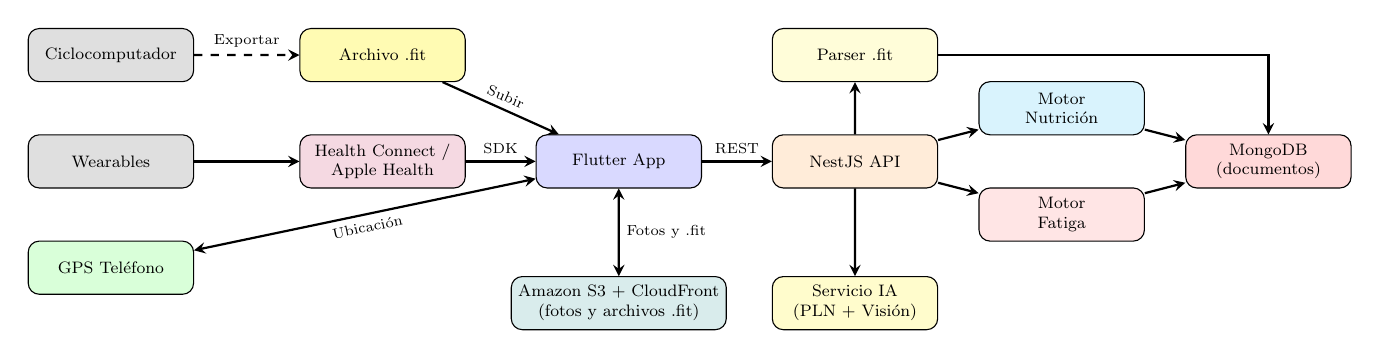
\begin{tikzpicture}[
    box/.style={draw, rectangle, rounded corners, minimum width=2.8cm, minimum height=0.9cm, fill=#1, align=center, font=\footnotesize},
    arrow/.style={->, thick, >=stealth},
    darrow/.style={<->, thick, >=stealth},
    dashed_arrow/.style={->, dashed, thick, >=stealth},
    lbl/.style={font=\scriptsize},
    scale=0.75, transform shape
]
    % Dispositivos del usuario
    \node (ciclo) [box=gray!25] at (-0.6,1.8) {Ciclocomputador};
    \node (wear) [box=gray!25] at (-0.6,0) {Wearables};
    \node (gps) [box=green!15] at (-0.6,-1.8) {GPS Teléfono};

    % Concentradores y archivo exportado
    \node (fit) [box=yellow!30] at (4,1.8) {Archivo .fit};
    \node (hc) [box=purple!15] at (4,0) {Health Connect /\\Apple Health};

    % Aplicación y almacenamiento de archivos
    \node (app) [box=blue!15] at (8,0) {Flutter App};
    \node (s3) [box=teal!15] at (8,-2.4) {Amazon S3 + CloudFront\\(fotos y archivos .fit)};

    % Backend
    \node (api) [box=orange!15] at (12,0) {NestJS API};
    \node (parser) [box=yellow!15] at (12,1.8) {Parser .fit};
    \node (ai) [box=yellow!20] at (12,-2.4) {Servicio IA\\(PLN + Visión)};
    \node (nutri) [box=cyan!15] at (15.5,0.9) {Motor\\Nutrición};
    \node (fatiga) [box=red!10] at (15.5,-0.9) {Motor\\Fatiga};

    % Base de datos
    \node (db) [box=red!15] at (19,0) {MongoDB\\(documentos)};

    % Flechas
    \draw[dashed_arrow] (ciclo) -- node[above, lbl] {Exportar} (fit);
    \draw[arrow] (wear) -- (hc);
    \draw[arrow] (fit) -- node[above, lbl, sloped] {Subir} (app);
    \draw[arrow] (hc) -- node[above, lbl] {SDK} (app);
    \draw[darrow] (gps) -- node[below, lbl, sloped] {Ubicación} (app);
    \draw[darrow] (app) -- node[right, lbl] {Fotos y .fit} (s3);
    \draw[arrow] (app) -- node[above, lbl] {REST} (api);
    \draw[arrow] (api) -- (parser);
    \draw[arrow] (api) -- (ai);
    \draw[arrow] (api) -- (nutri);
    \draw[arrow] (api) -- (fatiga);
    \draw[arrow] (nutri) -- (db);
    \draw[arrow] (fatiga) -- (db);
    \draw[arrow] (parser) -| (db);

\end{tikzpicture}
\captionof{figure}{Arquitectura de la Alternativa 3: Solución por Capas.}
\end{center}
\vspace{0.5cm}
\newpage
\textbf{Estimación de Costos}

La siguiente tabla resume los costos de esta alternativa. El costo de desarrollo viene del análisis por ciclo de vida (Tabla \ref{tab:ciclovida_alt3}), y los demás valores son los mismos que se usan en su flujo de caja dentro de la factibilidad económica.

\begin{table}[h!]
    \centering
    \renewcommand{\arraystretch}{1.4}
    \begin{tabular}{|m{4cm}|m{5.5cm}|r|}
        \hline
        \rowcolor[HTML]{EFEFEF}
        \textbf{Ítem} & \textbf{Detalle} & \textbf{Costo (CLP)} \\ \hline
        \multicolumn{3}{|l|}{\cellcolor[HTML]{E3F2FD}\textbf{Inversión inicial (Año 0)}} \\ \hline
        Desarrollo de software & 508 horas de trabajo según el ciclo de vida & \$16.109.800 \\ \hline
        Publicación en tiendas & Google Play y Apple Developer & \$120.602 \\ \hline
        \rowcolor[HTML]{E8F5E9}
        \textbf{Total inversión inicial} & & \textbf{\$16.230.402} \\ \hline
        \multicolumn{3}{|l|}{\cellcolor[HTML]{FFF3E0}\textbf{Costos operativos anuales (Años 1 a 4)}} \\ \hline
        Infraestructura Cloud & AWS (Fargate, Lambda, ALB, IP públicas, CloudWatch y S3 para archivos \texttt{.fit}) y MongoDB Atlas M10 (Tabla \ref{tab:costo_infra}) & \$2.124.158 \\ \hline
        Imágenes & S3 y CloudFront para las fotos de perfil y de las publicaciones (Tabla \ref{tab:costo_imagenes}) & \$70.027 \\ \hline
        APIs de IA & Gemini (uso anual) & \$641.916 \\ \hline
        Mantenimiento & 10\% del costo de desarrollo & \$1.610.980 \\ \hline
        Suscripción Apple & Renovación anual del Apple Developer Program & \$96.287 \\ \hline
        \rowcolor[HTML]{FFF3E0}
        \textbf{Total operativo anual} & & \textbf{\$4.543.368} \\ \hline
    \end{tabular}
    \caption{Estimación de costos de la Alternativa 3: Solución por Capas.}
    \label{tab:costos_alt3}
\end{table}

\textbf{Complejidad adicional:} Los registros de cardio llegan desde fuentes con niveles de detalle muy distintos (desde el GPS del teléfono hasta archivos \texttt{.fit} con miles de puntos). Para poder usarlos en conjunto hay que diseñar una base de datos flexible y un proceso que los deje en un formato común que el motor de fatiga pueda consultar.
\newpage
\subsubsection{Cuadro Comparativo de Alternativas}
La siguiente tabla resume las diferencias funcionales, técnicas y económicas entre las tres alternativas, como base para la elección que se hace en el estudio de factibilidad.

\begin{table}[h!]
    \centering
    \renewcommand{\arraystretch}{1.4}
    \begin{tabular}{|m{3.8cm}|m{3.5cm}|m{3.5cm}|m{3.8cm}|}
        \hline
        \rowcolor[HTML]{EFEFEF}
        \textbf{Dimensión} & \textbf{Alt. 1: Minimalista} & \textbf{Alt. 2: Brokers SO} & \textbf{Alt. 3: Por Capas} \\ \hline
        \textbf{Registro Nutricional} & Formulario manual & PLN + Visión IA & PLN + Visión IA + Escalado comunitario \\ \hline
        \textbf{Registro de Fuerza} & Formulario manual & Formulario + PLN & Formulario + PLN \\ \hline
        \textbf{Registro de Cardio} & GPS teléfono + RPE & GPS + Health Connect / Apple Health & GPS + Brokers + Archivo .fit \\ \hline
        \textbf{Frecuencia Cardíaca} & No disponible & Sí (vía broker) & Sí (broker + .fit segundo a segundo) \\ \hline
        \textbf{Potencia (ciclismo)} & No disponible & No disponible & Sí (vía archivo .fit) \\ \hline
        \textbf{Precisión del motor de fatiga} & Baja (volumen + RPE) & Media-Alta (zonas FC + calorías) & Alta (potencia + FC + TSS) \\ \hline
        \textbf{Módulo Social} & Básico (compartir) & Compartir con ajuste de recetas & Red social con contenido reutilizable en todos los módulos \\ \hline
        \textbf{Fotos que se guardan} & Solo perfil & Perfil y recetas & Perfil y publicaciones (hasta 4 por publicación) \\ \hline
        \textbf{Perfil y plan sugerido} & No & No & Sí \\ \hline
        \textbf{Uso de IA} & No & Sí (PLN + Visión) & Sí (PLN + Visión) \\ \hline
        \textbf{Tiempo de desarrollo} & 3-4 meses & 6-7 meses & 9-10 meses \\ \hline
        \textbf{Inversión inicial} & \$8.666.229 CLP & \$12.242.990 CLP & \$16.230.402 CLP \\ \hline
        \textbf{Costo operativo anual} & \$2.841.584 CLP & \$3.899.532 CLP & \$4.543.368 CLP \\ \hline
        \textbf{Complejidad técnica} & Baja & Media & Alta \\ \hline
        \textbf{Barrera de entrada usuario} & Ninguna (solo teléfono) & Baja (smartwatch opcional) & Ninguna (escala con hardware) \\ \hline
    \end{tabular}
    \caption{Cuadro comparativo de las alternativas de solución.}
    \label{tab:comparativa_alternativas}
\end{table}
\newpage
\subsection{Estudio de Factibilidad}
El estudio de factibilidad sirve para evaluar si la solución propuesta se puede llevar a cabo antes de invertir recursos en ella. Este análisis se divide en tres partes, que son la factibilidad técnica, la económica y la operativa. Con esta evaluación se busca identificar restricciones y riesgos a tiempo, y confirmar que se cuenta con la tecnología, el presupuesto y las condiciones necesarias para construir el sistema y desarrollar el Producto Mínimo Viable (MVP) con la alternativa elegida.

\subsubsection{Factibilidad Técnica}
La factibilidad técnica evalúa si se cuenta con la tecnología, la infraestructura y los conocimientos necesarios para desarrollar y mantener el sistema. Considerando que el proyecto integra varias fuentes de datos y usa inteligencia artificial, el análisis se hace desde los siguientes puntos de vista:
\newpage
\textbf{1. Disponibilidad del Stack Tecnológico:}\\
El sistema se basa en tecnologías maduras, de código abierto (open-source) y muy usadas en la industria. Esto reduce la dependencia de proveedores cerrados y facilita que el sistema pueda crecer más adelante.
\begin{itemize}
    \item Frontend: Flutter (mantenido por Google) tiene mucha documentación y una gran cantidad de paquetes de la comunidad (pub.dev) que facilitan el acceso al GPS, la cámara y el almacenamiento del teléfono, con un solo código para iOS y Android.
    \item Backend: NestJS, construido sobre Node.js y TypeScript, tiene una estructura por módulos que permite crear APIs REST y manejar servicios más complejos, como la lectura de archivos y los cálculos. Además, TypeScript es un lenguaje muy conocido, por lo que es fácil encontrar documentación y desarrolladores.
    \item Base de Datos: MongoDB es una de las bases de datos NoSQL más usadas. Cuenta con un servicio administrado en la nube (MongoDB Atlas), un driver oficial para Node.js y librerías como Mongoose que se integran con NestJS. Además, permite guardar series de tiempo de forma nativa, lo que sirve para la telemetría de los dispositivos. Las primeras pruebas del prototipo se hicieron con Firestore, otra base de datos orientada a documentos, y el modelo funcionó bien, lo que respalda este enfoque.
\end{itemize}

\textbf{2. Integración con Hardware y Concentradores (Brokers):}\\
Leer automáticamente los datos de cardio de los wearables es técnicamente posible. Tanto Google (con Health Connect) como Apple (con HealthKit) ofrecen Kits de Desarrollo de Software (SDKs) bien documentados, con los que una aplicación puede pedir permisos de lectura al usuario y acceder a datos como la frecuencia cardíaca, los pasos y las calorías. Además, Flutter cuenta con librerías de la comunidad que permiten usar ambas plataformas con un mismo código en Dart, lo que reduce bastante el trabajo de integración.
\newpage
\textbf{3. Inteligencia Artificial (PLN y Visión Artificial):}\\
Desarrollar y entrenar modelos propios de lenguaje natural o de reconocimiento de alimentos desde cero requeriría equipos con GPUs y especialistas en ciencia de datos, lo que haría inviable el MVP tanto en lo técnico como en lo económico.
\\\\
Sin embargo, usar APIs comerciales en la nube (como OpenAI, Google Gemini API o plataformas de análisis de alimentos como LogMeal) hace que esta función sea completamente factible. Estas plataformas funcionan como un servicio (AI as a Service). La aplicación solo tiene que enviar solicitudes HTTPS, el procesamiento pesado lo hacen los servidores del proveedor y la respuesta llega ordenada en formato JSON.
\\\\
\textbf{4. Procesamiento de Archivos .FIT:}\\
Leer archivos \texttt{.fit} de ciclocomputadores es factible porque el consorcio ANT+ publica su protocolo de forma abierta. Hoy existen varios paquetes de código abierto en lenguajes como JavaScript, TypeScript o Python que leen estos archivos binarios y los convierten en listas de datos para obtener la información segundo a segundo (potencia, cadencia). Por lo tanto, no es necesario programar el lector desde cero.
\\\\
\textbf{5. Red Social y Plan Sugerido:}\\
La red social se construye con funciones conocidas, como seguir usuarios, un muro de publicaciones paginado y la copia de una publicación al módulo de quien la ve. Las fotos de las publicaciones tampoco son un problema técnico. El teléfono las comprime antes de subirlas y las envía directamente a Amazon S3, el mismo almacenamiento de los archivos \texttt{.fit}, usando un permiso temporal que entrega el backend. En MongoDB solo queda su dirección, y para mostrarlas se usa Amazon CloudFront, que guarda copias cerca de los usuarios. Los videos se dejan para después del MVP, porque pesan mucho más y hay que procesarlos antes de mostrarlos. El plan sugerido tampoco exige técnicas complejas, ya que parte de plantillas definidas para cada perfil (nivel y orientación) que se ajustan con reglas simples según la adherencia, el RPE y la fatiga registrada.
\newpage
\textbf{Conclusión de Factibilidad Técnica:}\\
Se concluye que el proyecto es \textbf{técnicamente factible}. No requiere crear hardware nuevo, hacer descubrimientos científicos ni inventar algoritmos o lenguajes desde cero. La solución se basa en combinar servicios en la nube, SDKs públicos y frameworks que ya están probados, documentados y disponibles para cualquier desarrollador.

\subsubsection{Factibilidad Económica}
La factibilidad económica evalúa si el proyecto puede generar ingresos que justifiquen la inversión. Para cada alternativa se construye un flujo de caja proyectado a 4 años, y con él se calculan tres indicadores financieros, que son el Valor Actual Neto (VAN), la Tasa Interna de Retorno (TIR) y el Periodo de Recuperación de la Inversión (Payback).
\\\\
El objetivo es calcular, para cada alternativa, el \textbf{ingreso anual neto mínimo} con el que se logra al mismo tiempo un VAN igual a cero, una TIR del 15\% y un Payback dentro del cuarto año de operación.
\\\\
\textbf{Modelo de Ingresos}

La plataforma funcionará con un modelo de suscripción freemium. Habrá una versión gratuita con el registro manual y el plan sugerido, y para acceder a todo lo demás, que incluye la integración con wearables, la asistencia por IA, el cruce de datos, las alertas, las metas de alimentación y la red social, se deberá pagar una suscripción mensual premium. Tomando como referencia precios del mercado chileno (Fitia Premium a \$6.990 CLP al mes, Strava a \$7.600 CLP al mes y Freeletics a \$8.000 CLP al mes), se fija un precio de \textbf{\$7.990 CLP al mes}, es decir, \textbf{\$95.880 CLP al año} por usuario.
\\\\
Sin embargo, el proyecto no recibe ese monto completo. El precio incluye un IVA de 19\% \citep{sii_iva_digital}, por lo que sin IVA queda en \$6.714 CLP al mes. Además, el cobro se hace a través de Google Play y App Store, que cobran una comisión de hasta 15\% para desarrolladores con ingresos menores a un millón de dólares al año \citep{apple_small_business, google_service_fees}. Se considera el 15\% sobre el precio sin IVA, por lo que quedan \$5.707 CLP al mes por suscriptor. Es decir, el \textbf{ingreso neto por suscriptor es de \$68.486 CLP al año}, y este es el valor que se usa para calcular cuántos suscriptores se necesitan.
\newpage
\textbf{Breve Estudio Exploratorio de Mercado}

Para un producto enfocado en entrenamiento concurrente y nutrición, el tamaño del mercado en Chile se puede estimar de la siguiente forma \citep{mindep_habitos}:

\begin{itemize}
    \item \textbf{TAM (Mercado total, deportistas en Chile):} Según la Encuesta Nacional de Hábitos de Actividad Física y Deporte (MINDEP), entre el 32\% y el 35\% de la población mayor de 18 años hace actividad física de forma regular, lo que equivale a unos 4,5 a 5 millones de personas.
    \item \textbf{SAM (Mercado disponible, gimnasio, running y ciclismo):} Entre 1,2 y 1,5 millones de personas practican musculación, running o ciclismo. Dentro de este grupo, se estima que entre 180.000 y 250.000 personas hacen entrenamiento concurrente y usan smartphones junto con monitores de frecuencia cardíaca o GPS.
    \item \textbf{SOM (Mercado objetivo inicial):} Si se logra llegar a entre el 1\% y el 2\% del SAM en una primera etapa, se tendrían entre 1.800 y 5.000 usuarios activos. Para evaluar un escenario desfavorable, se considera una base de solo 1.500 usuarios, lo que equivale a menos del 1\% del SAM.
\end{itemize}

\vspace{0.3cm}
\textbf{El fenómeno de Hyrox y el atleta híbrido}

Las carreras de fitness híbrido, que combinan fuerza funcional con resistencia cardiovascular, son el mejor ejemplo de esta tendencia \citep{clarin_hyrox}.

\begin{itemize}
    \item La participación en Hyrox ha crecido muy rápido. Pasó de unos 650 competidores en su inicio en 2017 a más de 650.000 en 2024, y se proyecta que supere los 1,2 millones de atletas inscritos en la temporada 2025/2026 a nivel mundial.
    \item Un análisis de más de 275.000 atletas de esta modalidad mostró que atrae tanto a deportistas recreativos como de élite. Destaca la alta participación de personas mayores de 30 años y el crecimiento de la participación femenina, que ya ronda el 38\%.
    \item La preparación para estos eventos ha hecho que el entrenamiento concurrente se vuelva común en gimnasios tradicionales, donde los usuarios tienen que combinar sus sesiones de pesas con trabajo aeróbico intenso.
\end{itemize}

\vspace{0.3cm}
Además, el ACSM (American College of Sports Medicine), en su encuesta mundial de tendencias para 2026, mantiene al entrenamiento funcional y al uso de tecnología de datos (wearables) dentro de su Top 10. Según estos reportes, los usuarios se están alejando del enfoque solo estético y le dan más importancia a la funcionalidad, la longevidad y el rendimiento general \citep{acsm_trends}.
\\\\
Por su parte, el informe Year in Sport de Strava mostró que sus usuarios están probando cada vez más disciplinas distintas. El entrenamiento de fuerza fue la actividad que más creció entre las mujeres en la plataforma (con un aumento del 25\% en las actividades registradas), y al mismo tiempo la participación en clubes de running aumentó un 59\% \citep{strava_yis}.
\\\\
Por lo tanto, se concluye que una base inicial (SOM) de unos 1.500 posibles usuarios en Chile que hacen entrenamiento concurrente es razonable, y las fuentes indican que este número va en aumento.

\newpage
\textbf{Estimación de Costos por Ciclo de Vida del Desarrollo de Software}

Para respaldar los costos de desarrollo de cada alternativa, a continuación se presenta una estimación detallada basada en el ciclo de vida del software. El esfuerzo total se divide en cinco etapas. Las horas de trabajo (HH) se valorizaron con tarifas distintas según el cargo, obtenidas de una revisión del mercado laboral chileno en 2026 (portales como Computrabajo, Indeed e ITWorkers, entre otros). Estas tarifas van desde \textbf{\$12.320 CLP por hora} para asesores en la etapa de pruebas hasta \textbf{\$73.917 CLP por hora} para un Jefe de Proyecto Senior.

\begin{enumerate}
    \item \textbf{Análisis:} Levantamiento y especificación de los requerimientos funcionales y no funcionales, y definición del alcance y las restricciones del sistema.
    \item \textbf{Diseño Lógico:} Diseño de la arquitectura, modelo conceptual de la base de datos, definición de interfaces y API, y diseño de la experiencia de usuario (wireframes).
    \item \textbf{Diseño Físico:} Programación de todos los componentes del sistema, incluyendo frontend, backend, base de datos, integraciones y servicios de apoyo.
    \item \textbf{Pruebas QA:} Pruebas unitarias, de integración, funcionales y de rendimiento para asegurar la calidad del producto.
    \item \textbf{Implementación:} Configuración de la infraestructura, despliegue en la nube, publicación en las tiendas de aplicaciones y puesta en marcha del sistema.
\end{enumerate}
\newpage
\textbf{Ciclo de Vida de la Alternativa 1: Solución Minimalista}

\begin{table}[h!]
    \centering
    \renewcommand{\arraystretch}{1.15}
    \footnotesize
    \begin{tabular}{|l|c|r|r|r|}
        \hline
        \rowcolor[HTML]{EFEFEF}
        \textbf{Cargo} & \textbf{Cant.} & \textbf{Horas} & \textbf{VH (CLP)} & \textbf{Total (CLP)} \\ \hline
        \multicolumn{5}{|l|}{\cellcolor[HTML]{E3F2FD}\textbf{Etapa 1: Análisis}} \\ \hline
        JP Senior & 1 & 8 & \$73.917 & \$591.336 \\ \hline
        JP Junior & 1 & 6 & \$32.852 & \$197.112 \\ \hline
        Nutricionista/Coach Dep. (Asesor) & 1 & 6 & \$20.533 & \$123.195 \\ \hline
        \rowcolor[HTML]{F3F3F3}
        \multicolumn{4}{|r|}{\textbf{Subtotal Análisis}} & \textbf{\$911.643} \\ \hline
        \multicolumn{5}{|l|}{\cellcolor[HTML]{E3F2FD}\textbf{Etapa 2: Diseño Lógico}} \\ \hline
        JP Senior & 1 & 8 & \$73.917 & \$591.336 \\ \hline
        JP Junior & 1 & 14 & \$32.852 & \$459.928 \\ \hline
        Arquitecto Web & 1 & 24 & \$32.852 & \$788.448 \\ \hline
        Desarrollador UX/UI & 1 & 6 & \$28.746 & \$172.473 \\ \hline
        Nutricionista/Coach Dep. (Asesor) & 1 & 10 & \$12.320 & \$123.195 \\ \hline
        \rowcolor[HTML]{F3F3F3}
        \multicolumn{4}{|r|}{\textbf{Subtotal Diseño Lógico}} & \textbf{\$2.135.380} \\ \hline
        \multicolumn{5}{|l|}{\cellcolor[HTML]{E3F2FD}\textbf{Etapa 3: Diseño Físico}} \\ \hline
        JP Senior & 1 & 10 & \$73.917 & \$739.170 \\ \hline
        JP Junior & 1 & 10 & \$32.852 & \$328.520 \\ \hline
        Desarrollador UX/UI & 1 & 50 & \$28.746 & \$1.437.275 \\ \hline
        Desarrollador Backend & 1 & 50 & \$28.746 & \$1.437.275 \\ \hline
        Nutricionista/Coach Dep. (Asesor) & 1 & 6 & \$12.320 & \$73.917 \\ \hline
        \rowcolor[HTML]{F3F3F3}
        \multicolumn{4}{|r|}{\textbf{Subtotal Diseño Físico}} & \textbf{\$4.016.157} \\ \hline
        \multicolumn{5}{|l|}{\cellcolor[HTML]{E3F2FD}\textbf{Etapa 4: Pruebas QA}} \\ \hline
        JP Junior & 1 & 10 & \$32.852 & \$328.520 \\ \hline
        Ingeniero QA & 1 & 15 & \$24.639 & \$369.585 \\ \hline
        Nutricionista/Coach Dep. (Asesor) & 1 & 5 & \$12.320 & \$61.598 \\ \hline
        \rowcolor[HTML]{F3F3F3}
        \multicolumn{4}{|r|}{\textbf{Subtotal Pruebas QA}} & \textbf{\$759.703} \\ \hline
        \multicolumn{5}{|l|}{\cellcolor[HTML]{E3F2FD}\textbf{Etapa 5: Implementación}} \\ \hline
        JP Junior & 1 & 10 & \$32.852 & \$328.520 \\ \hline
        DevOps & 1 & 12 & \$32.852 & \$394.224 \\ \hline
        \rowcolor[HTML]{F3F3F3}
        \multicolumn{4}{|r|}{\textbf{Subtotal Implementación}} & \textbf{\$722.744} \\ \hline
        \rowcolor[HTML]{E8F5E9}
        \multicolumn{4}{|r|}{\textbf{TOTAL DESARROLLO PERSONAL}} & \textbf{\$8.545.627} \\ \hline
    \end{tabular}
    \caption{Desglose detallado de costos de personal por etapa: Alternativa 1.}
    \label{tab:ciclovida_alt1}
\end{table}
\newpage
\textbf{Ciclo de Vida de la Alternativa 2: Solución Integrada con Brokers}

\begin{table}[h!]
    \centering
    \renewcommand{\arraystretch}{1.15}
    \footnotesize
    \begin{tabular}{|l|c|r|r|r|}
        \hline
        \rowcolor[HTML]{EFEFEF}
        \textbf{Cargo} & \textbf{Cant.} & \textbf{Horas} & \textbf{VH (CLP)} & \textbf{Total (CLP)} \\ \hline
        \multicolumn{5}{|l|}{\cellcolor[HTML]{E3F2FD}\textbf{Etapa 1: Análisis}} \\ \hline
        JP Senior & 1 & 8 & \$73.917 & \$591.336 \\ \hline
        JP Junior & 1 & 6 & \$32.852 & \$197.112 \\ \hline
        Nutricionista/Coach Dep. (Asesor) & 1 & 6 & \$20.533 & \$123.195 \\ \hline
        Científico de Datos / IA & 1 & 6 & \$28.746 & \$172.473 \\ \hline
        \rowcolor[HTML]{F3F3F3}
        \multicolumn{4}{|r|}{\textbf{Subtotal Análisis}} & \textbf{\$1.084.116} \\ \hline
        \multicolumn{5}{|l|}{\cellcolor[HTML]{E3F2FD}\textbf{Etapa 2: Diseño Lógico}} \\ \hline
        JP Senior & 1 & 8 & \$73.917 & \$591.336 \\ \hline
        JP Junior & 1 & 14 & \$32.852 & \$459.928 \\ \hline
        Arquitecto Web & 1 & 28 & \$32.852 & \$919.856 \\ \hline
        Desarrollador UX/UI & 1 & 6 & \$28.746 & \$172.473 \\ \hline
        Nutricionista/Coach Dep. (Asesor) & 1 & 14 & \$12.320 & \$172.473 \\ \hline
        Científico de Datos / IA & 1 & 8 & \$28.746 & \$229.964 \\ \hline
        \rowcolor[HTML]{F3F3F3}
        \multicolumn{4}{|r|}{\textbf{Subtotal Diseño Lógico}} & \textbf{\$2.546.030} \\ \hline
        \multicolumn{5}{|l|}{\cellcolor[HTML]{E3F2FD}\textbf{Etapa 3: Diseño Físico}} \\ \hline
        JP Senior & 1 & 10 & \$73.917 & \$739.170 \\ \hline
        JP Junior & 1 & 14 & \$32.852 & \$459.928 \\ \hline
        Desarrollador UX/UI & 1 & 60 & \$28.746 & \$1.724.730 \\ \hline
        Desarrollador Backend & 1 & 60 & \$28.746 & \$1.724.730 \\ \hline
        Nutricionista/Coach Dep. (Asesor) & 1 & 6 & \$12.320 & \$73.917 \\ \hline
        Científico de Datos / IA & 1 & 30 & \$28.746 & \$862.365 \\ \hline
        Desarrollador Mobile & 1 & 30 & \$28.746 & \$862.365 \\ \hline
        Ingeniero DB & 1 & 15 & \$28.746 & \$431.183 \\ \hline
        \rowcolor[HTML]{F3F3F3}
        \multicolumn{4}{|r|}{\textbf{Subtotal Diseño Físico}} & \textbf{\$6.878.388} \\ \hline
        \multicolumn{5}{|l|}{\cellcolor[HTML]{E3F2FD}\textbf{Etapa 4: Pruebas QA}} \\ \hline
        JP Junior & 1 & 10 & \$32.852 & \$328.520 \\ \hline
        Ingeniero QA & 1 & 15 & \$24.639 & \$369.585 \\ \hline
        Nutricionista/Coach Dep. (Asesor) & 1 & 5 & \$12.320 & \$61.598 \\ \hline
        \rowcolor[HTML]{F3F3F3}
        \multicolumn{4}{|r|}{\textbf{Subtotal Pruebas QA}} & \textbf{\$759.703} \\ \hline
        \multicolumn{5}{|l|}{\cellcolor[HTML]{E3F2FD}\textbf{Etapa 5: Implementación}} \\ \hline
        JP Junior & 1 & 12 & \$32.852 & \$394.224 \\ \hline
        DevOps & 1 & 14 & \$32.852 & \$459.928 \\ \hline
        \rowcolor[HTML]{F3F3F3}
        \multicolumn{4}{|r|}{\textbf{Subtotal Implementación}} & \textbf{\$854.152} \\ \hline
        \rowcolor[HTML]{E8F5E9}
        \multicolumn{4}{|r|}{\textbf{TOTAL DESARROLLO PERSONAL}} & \textbf{\$12.122.388} \\ \hline
    \end{tabular}
    \caption{Desglose detallado de costos de personal por etapa: Alternativa 2.}
    \label{tab:ciclovida_alt2}
\end{table}

\newpage
\textbf{Ciclo de Vida de la Alternativa 3: Solución por Capas}

\begin{table}[h!]
    \centering
    \renewcommand{\arraystretch}{1.15}
    \footnotesize
    \begin{tabular}{|l|c|r|r|r|}
        \hline
        \rowcolor[HTML]{EFEFEF}
        \textbf{Cargo} & \textbf{Cant.} & \textbf{Horas} & \textbf{VH (CLP)} & \textbf{Total (CLP)} \\ \hline
        \multicolumn{5}{|l|}{\cellcolor[HTML]{E3F2FD}\textbf{Etapa 1: Análisis}} \\ \hline
        JP Senior & 1 & 14 & \$73.917 & \$1.034.838 \\ \hline
        JP Junior & 1 & 10 & \$32.852 & \$328.520 \\ \hline
        Nutricionista/Coach Dep. (Asesor) & 1 & 6 & \$20.533 & \$123.195 \\ \hline
        Científico de Datos / IA & 1 & 6 & \$28.746 & \$172.473 \\ \hline
        Esp. Telemetría Wearables & 1 & 6 & \$28.746 & \$172.473 \\ \hline
        \rowcolor[HTML]{F3F3F3}
        \multicolumn{4}{|r|}{\textbf{Subtotal Análisis}} & \textbf{\$1.831.499} \\ \hline
        \multicolumn{5}{|l|}{\cellcolor[HTML]{E3F2FD}\textbf{Etapa 2: Diseño Lógico}} \\ \hline
        JP Senior & 1 & 12 & \$73.917 & \$887.004 \\ \hline
        JP Junior & 1 & 20 & \$32.852 & \$657.040 \\ \hline
        Arquitecto Web & 1 & 32 & \$32.852 & \$1.051.264 \\ \hline
        Desarrollador UX/UI & 1 & 6 & \$28.746 & \$172.473 \\ \hline
        Nutricionista/Coach Dep. (Asesor) & 1 & 20 & \$12.320 & \$246.390 \\ \hline
        Científico de Datos / IA & 1 & 10 & \$28.746 & \$287.455 \\ \hline
        \rowcolor[HTML]{F3F3F3}
        \multicolumn{4}{|r|}{\textbf{Subtotal Diseño Lógico}} & \textbf{\$3.301.626} \\ \hline
        \multicolumn{5}{|l|}{\cellcolor[HTML]{E3F2FD}\textbf{Etapa 3: Diseño Físico}} \\ \hline
        JP Senior & 1 & 10 & \$73.917 & \$739.170 \\ \hline
        JP Junior & 1 & 20 & \$32.852 & \$657.040 \\ \hline
        Desarrollador UX/UI & 1 & 70 & \$28.746 & \$2.012.185 \\ \hline
        Desarrollador Backend & 1 & 70 & \$28.746 & \$2.012.185 \\ \hline
        Nutricionista/Coach Dep. (Asesor) & 1 & 6 & \$12.320 & \$73.917 \\ \hline
        Científico de Datos / IA & 1 & 40 & \$28.746 & \$1.149.820 \\ \hline
        Desarrollador Mobile & 1 & 35 & \$28.746 & \$1.006.093 \\ \hline
        Esp. Telemetría Wearables & 1 & 35 & \$28.746 & \$1.006.093 \\ \hline
        Ingeniero DB & 1 & 20 & \$28.746 & \$574.910 \\ \hline
        \rowcolor[HTML]{F3F3F3}
        \multicolumn{4}{|r|}{\textbf{Subtotal Diseño Físico}} & \textbf{\$9.231.412} \\ \hline
        \multicolumn{5}{|l|}{\cellcolor[HTML]{E3F2FD}\textbf{Etapa 4: Pruebas QA}} \\ \hline
        JP Junior & 1 & 10 & \$32.852 & \$328.520 \\ \hline
        Ingeniero QA & 1 & 15 & \$24.639 & \$369.585 \\ \hline
        Nutricionista/Coach Dep. (Asesor) & 1 & 5 & \$12.320 & \$61.598 \\ \hline
        \rowcolor[HTML]{F3F3F3}
        \multicolumn{4}{|r|}{\textbf{Subtotal Pruebas QA}} & \textbf{\$759.703} \\ \hline
        \multicolumn{5}{|l|}{\cellcolor[HTML]{E3F2FD}\textbf{Etapa 5: Implementación}} \\ \hline
        JP Junior & 1 & 14 & \$32.852 & \$459.928 \\ \hline
        DevOps & 1 & 16 & \$32.852 & \$525.632 \\ \hline
        \rowcolor[HTML]{F3F3F3}
        \multicolumn{4}{|r|}{\textbf{Subtotal Implementación}} & \textbf{\$985.560} \\ \hline
        \rowcolor[HTML]{E8F5E9}
        \multicolumn{4}{|r|}{\textbf{TOTAL DESARROLLO PERSONAL}} & \textbf{\$16.109.800} \\ \hline
    \end{tabular}
    \caption{Desglose detallado de costos de personal por etapa: Alternativa 3.}
    \label{tab:ciclovida_alt3}
\end{table}

\newpage
\textbf{Resumen Comparativo de Costos por Ciclo de Vida}

La siguiente tabla resume cómo se reparte el costo de personal en cada etapa del ciclo de vida para las tres alternativas.
\begin{table}[h!]
    \centering
    \renewcommand{\arraystretch}{1.4}
    \footnotesize
    \begin{tabular}{|m{2.8cm}|r|r|r|}
        \hline
        \rowcolor[HTML]{EFEFEF}
        \textbf{Etapa (miles CLP)} & \textbf{Alternativa 1} & \textbf{Alternativa 2} & \textbf{Alternativa 3} \\ \hline
        Análisis & \$912 & \$1.084& \$1.831 \\ \hline
        Diseño Lógico & \$2.135 & \$2.546 & \$3.302 \\ \hline
        Diseño Físico & \$4.016 & \$6.878 & \$9.231 \\ \hline
        Pruebas QA & \$760 & \$760 & \$760 \\ \hline
        Implementación & \$723 & \$854 & \$986 \\ \hline
        \rowcolor[HTML]{E8F5E9}
        \textbf{TOTAL} & \textbf{\$8.546} & \textbf{\$12.122} & \textbf{\$16.110} \\ \hline
    \end{tabular}
    \caption{Resumen comparativo de costos por ciclo de vida (valores en miles de CLP).}
    \label{tab:resumen_ciclovida}
\end{table}

\newpage
\textbf{Estructura de Costos: Inversión Inicial vs. Costos Operativos}

Para armar el flujo de caja, los costos se separan en dos grupos. El primero es la \textbf{inversión inicial} (Año 0), que incluye el desarrollo y la publicación inicial en las tiendas de aplicaciones. El segundo son los \textbf{costos operativos anuales} (Años 1 a 4), que incluyen la infraestructura en la nube (AWS Fargate, ALB y S3, junto con la base de datos administrada), el almacenamiento y la entrega de imágenes, el uso de APIs de IA (Gemini), la renovación del Apple Developer Program y un 10\% del costo de desarrollo para mantenimiento. Los videos no se consideran, porque quedan fuera del MVP.

\begin{table}[h!]
    \centering
    \renewcommand{\arraystretch}{1.4}
    \begin{tabular}{|m{4.5cm}|r|r|r|}
        \hline
        \rowcolor[HTML]{EFEFEF}
        \textbf{Concepto} & \textbf{Alt. 1} & \textbf{Alt. 2} & \textbf{Alt. 3} \\ \hline
        \multicolumn{4}{|l|}{\cellcolor[HTML]{E3F2FD}\textbf{Inversión Inicial (Año 0)}} \\ \hline
        Desarrollo de software & \$8.545.627 & \$12.122.388 & \$16.109.800 \\ \hline
        Publicación inicial tiendas & \$120.602 & \$120.602 & \$120.602 \\ \hline
        \rowcolor[HTML]{E8F5E9}
        \textbf{Total Inversión ($I_0$)} & \textbf{\$8.666.229} & \textbf{\$12.242.990} & \textbf{\$16.230.402} \\ \hline
        \multicolumn{4}{|l|}{\cellcolor[HTML]{FFF3E0}\textbf{Costos Operativos Anuales (Años 1--4)}} \\ \hline
        Infraestructura Cloud & \$1.879.063 & \$2.112.487 & \$2.124.158 \\ \hline
        Imágenes (S3 y CloudFront) & \$11.671 & \$11.671 & \$70.027 \\ \hline
        APIs de IA (Gemini) & --- & \$466.848 & \$641.916 \\ \hline
        Mantenimiento (10\% dev) & \$854.563 & \$1.212.239 & \$1.610.980 \\ \hline
        Suscripción Apple (anual) & \$96.287 & \$96.287 & \$96.287 \\ \hline
        \rowcolor[HTML]{FFF3E0}
        \textbf{Total Operativo ($C_{op}$)} & \textbf{\$2.841.584} & \textbf{\$3.899.532} & \textbf{\$4.543.368} \\ \hline
    \end{tabular}
    \caption{Desglose de costos por categoría para cada alternativa (en CLP).}
    \label{tab:desglose_costos}
\end{table}
\newpage
\textbf{Costo de la Infraestructura en la Nube}

La Tabla \ref{tab:costo_infra} detalla el costo de la infraestructura de cada alternativa. Se calculó con los precios publicados por AWS para la región de São Paulo \citep{aws_fargate_pricing}, y al tipo de cambio de \$972,60 CLP por dólar. Las tres alternativas usan un clúster MongoDB Atlas M10, porque es el nivel más bajo que permite una conexión privada con la red de AWS, algo necesario al trabajar con datos sensibles. Su precio en São Paulo es una estimación, ya que MongoDB publica USD 57 al mes para Virginia \citep{atlas_pricing}. El dimensionamiento de la alternativa elegida se explica en el capítulo de diseño.

\begin{table}[h!]
    \centering
    \renewcommand{\arraystretch}{1.25}
    \footnotesize
    \begin{tabular}{|>{\raggedright\arraybackslash}p{7.2cm}|r|r|r|}
        \hline
        \rowcolor[HTML]{EFEFEF}
        \textbf{Componente (USD al mes)} & \textbf{Alt. 1} & \textbf{Alt. 2} & \textbf{Alt. 3} \\ \hline
        API en Fargate (Alt. 1: 0,25 vCPU y 0,5 GB. Alt. 2 y 3: 0,5 vCPU y 1 GB) & 16 & 31 & 31 \\ \hline
        Parser \texttt{.fit} en Lambda, dentro del nivel gratuito & --- & --- & 0 \\ \hline
        MongoDB Atlas M10, con almacenamiento y respaldos & 100 & 100 & 100 \\ \hline
        Balanceador de carga (ALB) & 27 & 29 & 29 \\ \hline
        Direcciones IP públicas & 11 & 11 & 11 \\ \hline
        CloudWatch & 3 & 5 & 5 \\ \hline
        S3, sin contar las fotos & --- & 1 & 2 \\ \hline
        Secrets Manager, ECR y dominio & 4 & 4 & 4 \\ \hline
        \rowcolor[HTML]{FFF3E0}
        \textbf{Total infraestructura (USD al mes)} & \textbf{161} & \textbf{181} & \textbf{182} \\ \hline
        \rowcolor[HTML]{FFF3E0}
        \textbf{Total infraestructura (CLP al año)} & \textbf{\$1.879.063} & \textbf{\$2.112.487} & \textbf{\$2.124.158} \\ \hline
    \end{tabular}
    \caption{Costo de la infraestructura en la nube por alternativa.}
    \label{tab:costo_infra}
\end{table}
\newpage
\textbf{Costo de Almacenamiento y Entrega de Imágenes}

El costo de las fotos se estimó por separado, porque depende de cuántas imágenes guarda cada alternativa. Se usaron los precios de Amazon S3 en la región de São Paulo, que son USD 0,0405 por GB al mes y USD 0,007 por cada 1.000 subidas \citep{aws_s3_pricing}, y el nivel gratuito permanente de CloudFront, que incluye 1 TB de transferencia y 10 millones de solicitudes al mes \citep{aws_cloudfront_pricing}. Los supuestos son los siguientes:

\begin{itemize}
    \item Una base de 1.500 usuarios, igual al mercado objetivo inicial (SOM).
    \item Cada foto pesa unos 300 KB después de comprimirla, más una miniatura de 40 KB.
    \item En la Alternativa 2, el 10\% de los usuarios comparte 2 recetas con foto al mes.
    \item En la Alternativa 3, el 40\% de los usuarios publica 6 veces al mes con 2 fotos en promedio.
    \item Cada usuario ve unas 30 fotos al día en el muro, la mayoría como miniatura.
\end{itemize}

Como las fotos se acumulan, el costo crece año a año. Para tener un margen, se toma el costo del cuarto año, que es el más alto, se redondea hacia arriba y se aplica igual en todos los años.

\begin{table}[h!]
    \centering
    \renewcommand{\arraystretch}{1.4}
    \footnotesize
    \begin{tabular}{|>{\raggedright\arraybackslash}m{4.8cm}|>{\raggedright\arraybackslash}m{3cm}|>{\raggedright\arraybackslash}m{3cm}|>{\raggedright\arraybackslash}m{3.4cm}|}
        \hline
        \rowcolor[HTML]{EFEFEF}
        \textbf{Concepto} & \textbf{Alt. 1} & \textbf{Alt. 2} & \textbf{Alt. 3} \\ \hline
        Fotos que se guardan & Solo perfil & Perfil y recetas (1 foto) & Perfil y publicaciones (hasta 4 fotos) \\ \hline
        Fotos nuevas al mes & Solo nuevos perfiles & Unas 300 & Unas 7.200 \\ \hline
        Espacio acumulado al cuarto año & 0,4 GB & 5 GB & 118 GB \\ \hline
        Almacenamiento en S3 (USD/mes) & 0,02 & 0,2 & 4,8 \\ \hline
        Subidas a S3 (USD/mes) & 0,01 & 0,01 & 0,1 \\ \hline
        Entrega por CloudFront (USD/mes) & 0 & 0 & 0 (unos 110 GB y 1,4 millones de solicitudes al mes, dentro del nivel gratuito) \\ \hline
        \rowcolor[HTML]{FFF3E0}
        \textbf{Costo considerado (USD/mes)} & \textbf{1} & \textbf{1} & \textbf{6} \\ \hline
        \rowcolor[HTML]{FFF3E0}
        \textbf{Costo anual (CLP, a \$972,60 por USD)} & \textbf{\$11.671} & \textbf{\$11.671} & \textbf{\$70.027} \\ \hline
    \end{tabular}
    \caption{Estimación del costo de almacenamiento y entrega de imágenes.}
    \label{tab:costo_imagenes}
\end{table}

El costo de las imágenes es bajo incluso en la Alternativa 3, porque las fotos se comprimen en el teléfono y CloudFront entrega gratis el volumen esperado. Si la aplicación creciera mucho más allá del mercado objetivo, la entrega de fotos superaría el nivel gratuito, pero en ese escenario también habría muchos más suscriptores para cubrirla.
\newpage

\textbf{Formulación del Análisis Financiero}

Las tres métricas utilizadas se definen a continuación:

\begin{itemize}
    \item \textbf{Valor Actual Neto (VAN):} Es el valor que tienen hoy todos los flujos de caja futuros, descontados a una tasa $r$, menos la inversión inicial. Un VAN $\geq 0$ indica que el proyecto genera valor.
    \begin{equation}
        VAN = -I_0 + \sum_{t=1}^{n} \frac{FC_t}{(1+r)^t}
    \end{equation}

    \item \textbf{Tasa Interna de Retorno (TIR):} Es la tasa de descuento $r^*$ con la que el VAN queda exactamente en cero. Si la TIR es mayor que la tasa mínima que exige el inversionista, el proyecto es rentable.
    \begin{equation}
        0 = -I_0 + \sum_{t=1}^{n} \frac{FC_t}{(1+r^*)^t}
    \end{equation}

    \item \textbf{Periodo de Recuperación (Payback):} Es el tiempo que se demora la suma de los flujos netos en igualar la inversión inicial.
    \begin{equation}
        Payback = t \text{ tal que } \sum_{k=1}^{t} FC_k \geq I_0
    \end{equation}
\end{itemize}

\textbf{Impuesto a la Renta y Amortización}

Las utilidades del proyecto pagan el Impuesto de Primera Categoría, que en el régimen general es de un 27\% \citep{sii_tasas}. El impuesto se calcula sobre la utilidad, por lo que antes se puede descontar la inversión. El software hecho a medida no se deprecia como un activo físico, sino que se trata como un gasto diferido, que se puede amortizar hasta en seis años \citep{sii_software}. Aquí se amortiza toda la inversión inicial en partes iguales durante los 4 años del horizonte ($A = I_0 \div 4$). La amortización no es una salida real de dinero, así que se resta para calcular el impuesto y se vuelve a sumar para obtener el flujo neto.
\\\\
Se usa la tasa del régimen general porque es el caso más conservador. Una empresa pequeña podría acogerse al régimen Pro Pyme, que tiene una tasa menor \citep{sii_tasas}, lo que reduciría los suscriptores requeridos. Esta opción y la forma de amortizar se deben confirmar con un contador antes de operar.

\textbf{Cálculo del Ingreso Mínimo Requerido}

Para obtener el ingreso anual neto ($R$) que cumple las condiciones definidas (VAN = 0, TIR = 15\% y Payback $\leq$ 4 años), se parte del flujo de caja neto constante ($FC$) que recupera la inversión:
\begin{equation}
    FC = \frac{I_0}{\displaystyle\sum_{t=1}^{4} \frac{1}{(1{,}15)^t}} = \frac{I_0}{2{,}8550}
\end{equation}
Con el impuesto, el flujo neto es la utilidad después de impuesto más la amortización, es decir, $FC = (R - C_{op} - A)(1 - 0{,}27) + A$. Despejando el ingreso requerido se obtiene:
\begin{equation}
    R = C_{op} + A + \frac{FC - A}{1 - 0{,}27}
\end{equation}

\newpage
\textbf{Flujo de Caja Proyectado de la Alternativa 1: Solución Minimalista}

$FC_1 = 8.666.229 \div 2{,}8550 = \$3.035.457$ CLP/año.\\
Amortización anual: $A_1 = 8.666.229 \div 4 = \$2.166.557$ CLP/año.\\
Ingreso anual neto requerido por suscripciones:\\ $R_1 = 2.841.584 + 2.166.557 + (3.035.457 - 2.166.557) \div 0{,}73 = \$6.198.415$ CLP/año.




\begin{table}[h!]
    \centering
    \renewcommand{\arraystretch}{1.3}
    \footnotesize
    \begin{tabular}{|m{3.2cm}|r|r|r|r|r|}
        \hline
        \rowcolor[HTML]{EFEFEF}
        \textbf{Concepto (CLP)} & \textbf{Año 0} & \textbf{Año 1} & \textbf{Año 2} & \textbf{Año 3} & \textbf{Año 4} \\ \hline
        
        \textbf{Ingresos } &&&&&\\ \hline
        Suscripciones (neto) & --- & 6.198.415 & 6.198.415 & 6.198.415 & 6.198.415 \\ \hline
        \rowcolor[HTML]{E8F5E9}
        \textbf{Total Ingresos} & --- & 6.198.415 & 6.198.415 & 6.198.415 & 6.198.415 \\ \hline
        & & & & & \\ \hline
        \textbf{Egresos} & & & & & \\ \hline
        Infraestructura & --- & -1.879.063 & -1.879.063 & -1.879.063 & -1.879.063 \\ \hline
        Imágenes & --- & -11.671 & -11.671 & -11.671 & -11.671 \\ \hline
        APIs de IA & --- & --- & --- & --- & --- \\ \hline
        Mantenimiento & --- & -854.563 & -854.563 & -854.563 & -854.563 \\ \hline
        Apple Developer & --- & -96.287 & -96.287 & -96.287 & -96.287 \\ \hline
        \rowcolor[HTML]{F3E5F5}
        \textbf{Total Egresos} & --- & -2.841.584 & -2.841.584 & -2.841.584 & -2.841.584 \\ \hline
        & & & & & \\ \hline
        Amortización & --- & -2.166.557 & -2.166.557 & -2.166.557 & -2.166.557 \\ \hline
        \textbf{Utilidad antes de impuesto} & --- & \textbf{1.190.274} & \textbf{1.190.274} & \textbf{1.190.274} & \textbf{1.190.274} \\ \hline
        Impuesto (27\%) & --- & -321.374 & -321.374 & -321.374 & -321.374 \\ \hline
        \textbf{Utilidad después de impuesto} & --- & \textbf{868.900} & \textbf{868.900} & \textbf{868.900} & \textbf{868.900} \\ \hline
        Suma de la amortización & --- & 2.166.557 & 2.166.557 & 2.166.557 & 2.166.557 \\ \hline
        & & & & & \\ \hline
        Valor Desarrollo & -8.545.627 & --- & --- & --- & --- \\ \hline
        Valor Publicación & -120.602 & --- & --- & --- & --- \\ \hline
        \rowcolor[HTML]{F3E5F5} 
        Inversión Inicial & -8.666.229 & --- & --- & --- & --- \\ \hline
        & & & & & \\ \hline
        \rowcolor[HTML]{E8F5E9}
        \textbf{Flujo Neto} & \textbf{-8.666.229} & \textbf{3.035.457} & \textbf{3.035.457} & \textbf{3.035.457} & \textbf{3.035.457} \\ \hline
        Flujo Acumulado & -8.666.229 & -5.630.772 & -2.595.315 & 440.142 & 3.475.599 \\ \hline
        \rowcolor[HTML]{F3E5F5}
        Factor $(1{,}15)^{-t}$ & 1,000 & 0,870 & 0,756 & 0,658 & 0,572 \\ \hline
        \rowcolor[HTML]{F3E5F5}
        Flujo Descontado & -8.666.229 & 2.639.528 & 2.295.242 & 1.995.862 & 1.735.532 \\ \hline
    \end{tabular}
    \caption{Flujo de caja a 4 años - Alternativa 1.}
    \label{tab:flujo_alt1}
\end{table}

\begin{center}
\begin{tabular}{lll}
    $VAN_{15\%}$ = \$0 CLP \quad & $TIR$ = \textbf{15,0\%} \quad & $Payback$ = \textbf{2,85 años}
\end{tabular}
\end{center}

Suscriptores pagos requeridos: $6.198.415 \div 68.486 = 90,51$, lo que se redondea hacia arriba a \textbf{91 usuarios premium/año} para alcanzar el equilibrio.
Esto representa un \textbf{6,07\%} de la base conservadora de 1.500 posibles usuarios (SOM).

\newpage
\textbf{Flujo de Caja Proyectado de la Alternativa 2: Solución Integrada con Brokers}

$FC_2 = 12.242.990 \div 2{,}8550 = \$4.288.263$ CLP/año.\\
Amortización anual: $A_2 = 12.242.990 \div 4 = \$3.060.748$ CLP/año.\\
Ingreso anual neto requerido por suscripciones:\\ $R_2 = 3.899.532 + 3.060.748 + (4.288.263 - 3.060.748) \div 0{,}73 = \$8.641.807$ CLP/año.

\begin{table}[h!]
    \centering
    \renewcommand{\arraystretch}{1.3}
    \footnotesize
    \begin{tabular}{|m{3.2cm}|r|r|r|r|r|}
        \hline
        \rowcolor[HTML]{EFEFEF}
        \textbf{Concepto (CLP)} & \textbf{Año 0} & \textbf{Año 1} & \textbf{Año 2} & \textbf{Año 3} & \textbf{Año 4} \\ \hline
        
        \textbf{Ingresos } &&&&&\\ \hline
        Suscripciones (neto) & --- & 8.641.807 & 8.641.807 & 8.641.807 & 8.641.807 \\ \hline
        \rowcolor[HTML]{E8F5E9}
        \textbf{Total Ingresos} & --- & 8.641.807 & 8.641.807 & 8.641.807 & 8.641.807 \\ \hline
        & & & & & \\ \hline
        \textbf{Egresos} & & & & & \\ \hline
        Infraestructura & --- & -2.112.487 & -2.112.487 & -2.112.487 & -2.112.487 \\ \hline
        Imágenes & --- & -11.671 & -11.671 & -11.671 & -11.671 \\ \hline
        APIs de IA & --- & -466.848 & -466.848 & -466.848 & -466.848 \\ \hline
        Mantenimiento & --- & -1.212.239 & -1.212.239 & -1.212.239 & -1.212.239 \\ \hline
        Apple Developer & --- & -96.287 & -96.287 & -96.287 & -96.287 \\ \hline
        \rowcolor[HTML]{F3E5F5}
        \textbf{Total Egresos} & --- & -3.899.532 & -3.899.532 & -3.899.532 & -3.899.532 \\ \hline
        & & & & & \\ \hline
        Amortización & --- & -3.060.748 & -3.060.748 & -3.060.748 & -3.060.748 \\ \hline
        \textbf{Utilidad antes de impuesto} & --- & \textbf{1.681.527} & \textbf{1.681.527} & \textbf{1.681.527} & \textbf{1.681.527} \\ \hline
        Impuesto (27\%) & --- & -454.012 & -454.012 & -454.012 & -454.012 \\ \hline
        \textbf{Utilidad después de impuesto} & --- & \textbf{1.227.515} & \textbf{1.227.515} & \textbf{1.227.515} & \textbf{1.227.515} \\ \hline
        Suma de la amortización & --- & 3.060.748 & 3.060.748 & 3.060.748 & 3.060.748 \\ \hline
        & & & & & \\ \hline
        Valor Desarrollo & -12.122.388 & --- & --- & --- & --- \\ \hline
        Valor Publicación & -120.602 & --- & --- & --- & --- \\ \hline
        \rowcolor[HTML]{F3E5F5} 
        Inversión Inicial & -12.242.990 & --- & --- & --- & --- \\ \hline
        & & & & & \\ \hline
        \rowcolor[HTML]{E8F5E9}
        \textbf{Flujo Neto} & \textbf{-12.242.990} & \textbf{4.288.263} & \textbf{4.288.263} & \textbf{4.288.263} & \textbf{4.288.263} \\ \hline
        Flujo Acumulado & -12.242.990 & -7.954.727 & -3.666.464 & 621.799 & 4.910.062 \\ \hline
        \rowcolor[HTML]{F3E5F5}
        Factor $(1{,}15)^{-t}$ & 1,000 & 0,870 & 0,756 & 0,658 & 0,572 \\ \hline
        \rowcolor[HTML]{F3E5F5}
        Flujo Descontado & -12.242.990 & 3.728.924 & 3.242.543 & 2.819.603 & 2.451.828 \\ \hline
    \end{tabular}
    \caption{Flujo de caja a 4 años - Alternativa 2.}
    \label{tab:flujo_alt2}
\end{table}

\begin{center}
\begin{tabular}{lll}
    $VAN_{15\%}$ = \$0 CLP \quad & $TIR$ = \textbf{15,0\%} \quad & $Payback$ = \textbf{2,85 años}
\end{tabular}
\end{center}

Suscriptores pagos requeridos: $8.641.807 \div 68.486 = 126,18$, lo que se redondea hacia arriba a \textbf{127 usuarios premium/año} para alcanzar el equilibrio.
Esto representa un \textbf{8,47\%} de la base conservadora de 1.500 posibles usuarios (SOM).

\newpage
\textbf{Flujo de Caja Proyectado de la Alternativa 3: Solución por Capas}

$FC_3 = 16.230.402 \div 2{,}8550 = \$5.684.904$ CLP/año.\\
Amortización anual: $A_3 = 16.230.402 \div 4 = \$4.057.601$ CLP/año.\\
Ingreso anual neto requerido por suscripciones:\\ $R_3 = 4.543.368 + 4.057.601 + (5.684.904 - 4.057.601) \div 0{,}73 = \$10.830.151$ CLP/año.

\begin{table}[h!]
    \centering
    \renewcommand{\arraystretch}{1.3}
    \footnotesize
    \begin{tabular}{|m{3.2cm}|r|r|r|r|r|}
        \hline
        \rowcolor[HTML]{EFEFEF}
        \textbf{Concepto (CLP)} & \textbf{Año 0} & \textbf{Año 1} & \textbf{Año 2} & \textbf{Año 3} & \textbf{Año 4} \\ \hline
        
        \textbf{Ingresos } &&&&&\\ \hline
        Suscripciones (neto) & --- & 10.830.151 & 10.830.151 & 10.830.151 & 10.830.151 \\ \hline
        \rowcolor[HTML]{E8F5E9}
        \textbf{Total Ingresos} & --- & 10.830.151 & 10.830.151 & 10.830.151 & 10.830.151 \\ \hline
        & & & & & \\ \hline
        \textbf{Egresos} & & & & & \\ \hline
        Infraestructura & --- & -2.124.158 & -2.124.158 & -2.124.158 & -2.124.158 \\ \hline
        Imágenes & --- & -70.027 & -70.027 & -70.027 & -70.027 \\ \hline
        APIs de IA & --- & -641.916 & -641.916 & -641.916 & -641.916 \\ \hline
        Mantenimiento & --- & -1.610.980 & -1.610.980 & -1.610.980 & -1.610.980 \\ \hline
        Apple Developer & --- & -96.287 & -96.287 & -96.287 & -96.287 \\ \hline
        \rowcolor[HTML]{F3E5F5}
        \textbf{Total Egresos} & --- & -4.543.368 & -4.543.368 & -4.543.368 & -4.543.368 \\ \hline
        & & & & & \\ \hline
        Amortización & --- & -4.057.601 & -4.057.601 & -4.057.601 & -4.057.601 \\ \hline
        \textbf{Utilidad antes de impuesto} & --- & \textbf{2.229.182} & \textbf{2.229.182} & \textbf{2.229.182} & \textbf{2.229.182} \\ \hline
        Impuesto (27\%) & --- & -601.879 & -601.879 & -601.879 & -601.879 \\ \hline
        \textbf{Utilidad después de impuesto} & --- & \textbf{1.627.303} & \textbf{1.627.303} & \textbf{1.627.303} & \textbf{1.627.303} \\ \hline
        Suma de la amortización & --- & 4.057.601 & 4.057.601 & 4.057.601 & 4.057.601 \\ \hline
        & & & & & \\ \hline
        Valor Desarrollo & -16.109.800 & --- & --- & --- & --- \\ \hline
        Valor Publicación & -120.602 & --- & --- & --- & --- \\ \hline
        \rowcolor[HTML]{F3E5F5} 
        Inversión Inicial & -16.230.402 & --- & --- & --- & --- \\ \hline
        & & & & & \\ \hline
        \rowcolor[HTML]{E8F5E9}
        \textbf{Flujo Neto} & \textbf{-16.230.402} & \textbf{5.684.904} & \textbf{5.684.904} & \textbf{5.684.904} & \textbf{5.684.904} \\ \hline
        Flujo Acumulado & -16.230.402 & -10.545.498 & -4.860.594 & 824.310 & 6.509.214 \\ \hline
        \rowcolor[HTML]{F3E5F5}
        Factor $(1{,}15)^{-t}$ & 1,000 & 0,870 & 0,756 & 0,658 & 0,572 \\ \hline
        \rowcolor[HTML]{F3E5F5}
        Flujo Descontado & -16.230.402 & 4.943.395 & 4.298.604 & 3.737.917 & 3.250.362 \\ \hline
    \end{tabular}
    \caption{Flujo de caja a 4 años - Alternativa 3.}
    \label{tab:flujo_alt3}
\end{table}

\begin{center}
\begin{tabular}{lll}
    $VAN_{15\%}$ = \$0 CLP \quad & $TIR$ = \textbf{15,0\%} \quad & $Payback$ = \textbf{2,85 años}
\end{tabular}
\end{center}

Suscriptores pagos requeridos: $10.830.151 \div 68.486 = 158,14$, lo que se redondea hacia arriba a \textbf{159 usuarios premium/año} para alcanzar el equilibrio.
Esto representa un \textbf{10,60\%} de la base conservadora de 1.500 posibles usuarios (SOM).

\newpage
\textbf{Resumen Comparativo de Indicadores Financieros (Horizonte 4 años)}

\begin{table}[h!]
    \centering
    \renewcommand{\arraystretch}{1.5}
    \begin{tabular}{|m{4.5cm}|r|r|r|}
        \hline
        \rowcolor[HTML]{EFEFEF}
        \textbf{Indicador} & \textbf{Alt. 1} & \textbf{Alt. 2} & \textbf{Alt. 3} \\ \hline
        Inversión Inicial (CLP) & \$8.666.229 & \$12.242.990 & \$16.230.402 \\ \hline
        Costos Operativos/año (CLP) & \$2.841.584 & \$3.899.532 & \$4.543.368 \\ \hline
        Impuesto a la renta/año (CLP) & \$321.374 & \$454.012 & \$601.879 \\ \hline
        Ingreso neto mínimo/año (CLP) & \$6.198.415 & \$8.641.807 & \$10.830.151 \\ \hline
        Flujo Neto anual (CLP) & \$3.035.457 & \$4.288.263 & \$5.684.904 \\ \hline
        Ingreso neto por suscriptor/año (CLP) & \$68.486 & \$68.486 & \$68.486 \\ \hline
        VAN (al 15\%) & $\approx$ \$0 & $\approx$ \$0 & $\approx$ \$0 \\ \hline
        TIR & 15,0\% & 15,0\% & 15,0\% \\ \hline
        Payback (Flujo Acumulado) & 2,85 años & 2,85 años & 2,85 años \\ \hline
        \rowcolor[HTML]{E8F5E9}
        \textbf{Suscriptores requeridos} & \textbf{91} & \textbf{127} & \textbf{159} \\ \hline
        Mercado Objetivo Inicial (SOM) & 1.500 & 1.500 & 1.500 \\ \hline
        \rowcolor[HTML]{E8F5E9}
        \textbf{\% de conversión necesario} & \textbf{6,07\%} & \textbf{8,47\%} & \textbf{10,60\%} \\ \hline
    \end{tabular}
    \caption{Resumen de indicadores financieros por alternativa (Horizonte 4 años).}
    \label{tab:resumen_financiero}
\end{table}

\textbf{Conclusión de Factibilidad Económica}

Las tres alternativas son \textbf{económicamente factibles} con un horizonte de recuperación de 4 años, logrando una TIR del 15\% y un VAN en equilibrio. El análisis, hecho con tarifas del mercado chileno, muestra que la diferencia de costos entre alternativas es menor de lo que se esperaba al principio. Después de descontar el IVA, la comisión de las tiendas y el impuesto a la renta, la Alternativa 1 necesita 91 suscriptores premium para ser viable, la Alternativa 2 necesita 127 y la Alternativa 3 necesita 159 suscriptores al año. Con una base (SOM) estimada en 1.500 usuarios, llegar a 159 suscriptores implica una tasa de conversión del 10,6\%. Es una meta exigente para esa base conservadora, pero la conversión baja a un 8,8\% con 1.800 usuarios y a un 3,2\% con 5.000, que son los extremos del mercado objetivo inicial, por lo que se considera alcanzable. La Alternativa 3, al automatizar más el registro y aprovechar datos más detallados (archivos \texttt{.fit}), es la que más valor entrega al usuario y la que tiene más posibilidades de que este siga usando la aplicación en el tiempo.
\newpage
\newpage
\subsubsection{Factibilidad Operativa y Cumplimiento Normativo}
La factibilidad operativa evalúa si la solución se puede poner en marcha y operar en el entorno real para el que fue pensada, sin entrar en conflicto con las normas y leyes vigentes. Como la plataforma recolecta y cruza datos biológicos y de hábitos de los usuarios, su funcionamiento en Chile depende directamente del marco legal.
\\\\
A continuación se revisa cómo el proyecto cumple con las leyes chilenas que le aplican:

\textbf{1. Protección de Datos Personales y Datos Sensibles}\\
La aplicación guarda datos de los dispositivos (frecuencia cardíaca, ubicación GPS) y datos corporales (peso, consumo de calorías). Según la Ley N° 19.628 sobre Protección de la Vida Privada \citep{ley19628}, este tipo de información corresponde a datos sensibles.
\\\\
Por eso, el sistema incluirá lo siguiente:
\begin{itemize}
    \item Consentimiento explícito: Durante el registro inicial (onboarding), el usuario deberá autorizar de forma informada y clara el uso de sus datos antes de activar los permisos de lectura de Health Connect o Apple Health.
    \item Derechos ARCO: En la configuración de la cuenta, el usuario podrá ejercer sus derechos de Acceso, Rectificación, Cancelación y Oposición sobre sus datos. Esto incluye un botón de ``Eliminación de cuenta'' que borra todos los documentos asociados a su cuenta en la base de datos MongoDB.
    \item Principio de Finalidad: Los términos de uso indicarán que los datos solo se usan para calcular la fatiga y entregar sugerencias dentro de la aplicación, y que nunca se venderán ni se cederán perfiles fisiológicos a terceros.
    \item Privacidad en la red social: El usuario elegirá si cada publicación es pública, solo para sus seguidores o privada. En las rutas publicadas se ocultarán el inicio y el final del recorrido, para no revelar dónde vive o trabaja. Por el mismo motivo, antes de subir una foto la aplicación le borrará los datos de ubicación que guarda el teléfono.
\end{itemize}
\newpage
\textbf{2. Ciberseguridad y Gestión de Incidentes}\\
Como la aplicación móvil, la API en NestJS y los servicios de IA en la nube están en comunicación constante, el sistema debe cumplir con la Ley N° 21.459 sobre Delitos Informáticos \citep{ley21459} y con la Ley Marco de Ciberseguridad (Ley N° 21.663) \citep{ley21663}.
\\\\
Para operar de forma segura, toda la comunicación usará protocolos cifrados (HTTPS/TLS). Además, en la base de datos, los campos que guarden credenciales o tokens de acceso a servicios externos (como Garmin Connect o Apple) se almacenarán cifrados, para protegerlos en caso de que alguien intercepte la red o acceda a los datos.
\\\\
\textbf{3. Delimitación Sanitaria y Responsabilidad Civil}\\
La aplicación cruza los datos de fatiga para sugerir cambios en la alimentación y en las cargas de entrenamiento. Sin embargo, en Chile el Código Sanitario (DFL N° 725) \citep{dfl725} y la Ley N° 20.584 sobre Derechos y Deberes de los Pacientes \citep{ley20584} establecen que el diagnóstico clínico, la prescripción médica y la planificación de dietas terapéuticas son exclusivos de profesionales de la salud titulados.
\\\\
Para evitar riesgos legales, como el ejercicio ilegal de la profesión, la aplicación mostrará un aviso legal (disclaimer) obligatorio durante el registro. Este aviso dejará claro que la plataforma es una herramienta de ``apoyo deportivo para atletas aficionados sanos'' y que ninguna sugerencia de la aplicación reemplaza la indicación de un médico o nutricionista. Del mismo modo, el plan de entrenamiento sugerido y las metas de alimentación son orientaciones generales. La aplicación no entrega dietas ni planes de alimentación prescritos.
\newpage
\textbf{4. Comercio Electrónico y Modelo de Suscripción}\\
Como el modelo de ingresos se basa en una suscripción premium mensual de \$7.990 CLP, la parte comercial se rige por la Ley N° 19.496 sobre Protección de los Derechos de los Consumidores \citep{ley19496} y por el Reglamento de Comercio Electrónico (Decreto N° 6 del Ministerio de Economía).
\\\\
Esto exige transparencia total. La aplicación debe mostrar el precio final con impuestos incluidos y cada cuánto se cobra. Además, el usuario debe poder cancelar la suscripción desde la propia aplicación. Esta lo lleva a la pantalla de suscripciones de Google Play o App Store, donde confirma la cancelación sin necesidad de hablar con una persona.
\\\\
\textbf{5. Propiedad Intelectual y Licenciamiento}\\
El código fuente de la aplicación (Flutter y NestJS) queda protegido por la Ley N° 17.336 sobre Propiedad Intelectual \citep{ley17336}. Además, como la red social permite que los usuarios compartan sesiones, rutas, comidas, recetas y fotos, los términos de servicio incluirán una cláusula de licencia de uso no exclusiva, para que la aplicación pueda mostrar este contenido al resto de la comunidad y permitir que otros lo agreguen a sus módulos sin infringir derechos de autor. Al subir una foto, el usuario declarará que es suya o que tiene permiso para publicarla, y el administrador podrá retirar las que incumplan las normas de la comunidad. También se mantendrá un registro de las licencias open-source (MIT, Apache 2.0) de las librerías utilizadas (como el lector de archivos \texttt{.fit}), para cumplir con ellas al publicar en las tiendas de aplicaciones.
\newpage
\begin{table}[h!]
    \centering
    \renewcommand{\arraystretch}{1.5}
    \begin{tabular}{|m{3.5cm}|m{4cm}|m{7cm}|}
        \hline
        \rowcolor[HTML]{EFEFEF}
        \textbf{Dominio} & \textbf{Norma Chilena} & \textbf{Requisito Operativo en el Sistema} \\ \hline
        \textbf{Privacidad de Salud} & Ley N° 19.628 & Consentimiento explícito para biomarcadores y borrado total de cuenta. \\ \hline
        \textbf{Seguridad de Datos} & Leyes N° 21.459 y 21.663 & Cifrado SSL/TLS y protección en reposo para credenciales. \\ \hline
        \textbf{Ámbito Médico} & DFL N° 725 y Ley 20.584 & Disclaimer visible: la app no realiza prescripción clínica. \\ \hline
        \textbf{Monetización} & Ley N° 19.496 y Dcto. 6 & Transparencia de cobros y cancelación de la suscripción desde la aplicación. \\ \hline
        \textbf{Software y UGC} & Ley N° 17.336 & Términos de cesión para compartir sesiones, rutas, recetas y fotos en la comunidad. \\ \hline
    \end{tabular}
    \caption{Resumen del marco normativo y requisitos operativos.}
    \label{tab:resumen_normativo}
\end{table}

\textbf{Conclusión de Factibilidad Operativa:}\\
La plataforma es \textbf{operativamente factible}. Aunque trabajar con datos sensibles de salud implica un riesgo alto, los requisitos legales chilenos se pueden cumplir con decisiones de diseño incluidas desde el Producto Mínimo Viable, como el cifrado, la cancelación de la suscripción desde la aplicación, los avisos legales y el manejo de consentimientos.
\newpage
\subsubsection{Resumen del Estudio de Factibilidad y Selección de Alternativa}
Después de evaluar el proyecto en sus tres dimensiones (técnica, económica y operativa), se concluye que está en condiciones de avanzar a la etapa de diseño e implementación.
\\\\
En lo \textbf{técnico}, se cuenta con herramientas open-source probadas y con plataformas de IA en la nube, por lo que no es necesario inventar nada desde cero. En lo \textbf{operativo}, se confirmó que es posible ajustar el funcionamiento de la plataforma al marco legal chileno sobre datos sensibles, ciberseguridad y derechos del consumidor.
\\\\
En lo \textbf{económico}, el análisis muestra que el proyecto es rentable (VAN $\approx$ 0 y TIR del 15\%) con una cantidad acotada de usuarios de pago (hasta 159 suscriptores para la alternativa más compleja). Hay que tener en cuenta que estos cálculos no incluyen el Costo de Adquisición de Clientes (CAC) ni las campañas de marketing necesarias para llegar a esos usuarios. Aun considerando que el marketing tendría que financiarse por separado, la cantidad de suscriptores necesaria es acotada, por lo que la viabilidad comercial es favorable.
\\\\
\textbf{Decisión de arquitectura:} Según estos resultados, se decide \textbf{seleccionar la Alternativa 3 (Solución por Capas)} como arquitectura del proyecto. Aunque tiene la mayor inversión inicial, conseguir 159 usuarios premium dentro del nicho de entrenamiento híbrido en Chile es una meta alcanzable. Además, es la única alternativa que cubre el problema completo, porque automatiza el registro, puede crecer según el equipamiento del usuario y usa inteligencia artificial para facilitar el uso diario.
\newpage
\subsection{Solución a Implementar}
La solución a implementar se basa en la \textbf{Alternativa 3 (Solución por Capas)}, elegida porque permite reunir en un solo lugar el seguimiento del rendimiento físico y de la nutrición en el entrenamiento concurrente, combinando datos de dispositivos e inteligencia artificial.
\\\\
A continuación se describe la arquitectura técnica, los módulos funcionales, cómo se relacionan entre sí y el modelo de datos del Producto Mínimo Viable (MVP).
\newpage
\subsubsection{Visión General de la Arquitectura Lógica}
El sistema sigue un patrón Cliente-Servidor con una API REST. Está compuesto por los siguientes componentes:
\begin{itemize}
    \item \textbf{Frontend (Cliente Móvil):} Aplicación desarrollada en \textbf{Flutter} (Dart) para iOS y Android. Se encarga de la interfaz de usuario, del ingreso manual de datos, de usar el hardware del teléfono (cámara para fotos de comida y GPS para rutas) y de pedir los permisos para acceder a los datos de salud.
    \item \textbf{Backend (Servidor):} Desarrollado en \textbf{NestJS} (Node.js con TypeScript). Funciona como el punto central del sistema (BFF, Backend for Frontend). Procesa la lógica de negocio, hace los cálculos de fatiga, se encarga de la seguridad y conecta la aplicación con la base de datos y los servicios externos.
    \item \textbf{Base de Datos:} Se usará \textbf{MongoDB}, una base de datos NoSQL orientada a documentos. Permite guardar en una misma base datos con estructura simple (perfiles de usuario) y datos muy variables (sesiones de entrenamiento y series de tiempo de los wearables), sin tener que definir antes una estructura rígida.
    \item \textbf{Servicios Externos (Integraciones):} La API de Google Gemini, con sus modelos Flash, para el procesamiento de lenguaje natural y la visión artificial, Amazon S3 para guardar los archivos \texttt{.fit} y las fotos, Amazon CloudFront para mostrar las fotos de forma rápida, y los concentradores del sistema operativo (Health Connect y Apple HealthKit).
\end{itemize}

\vspace{0.5cm}
\begin{center}
\setstretch{1}
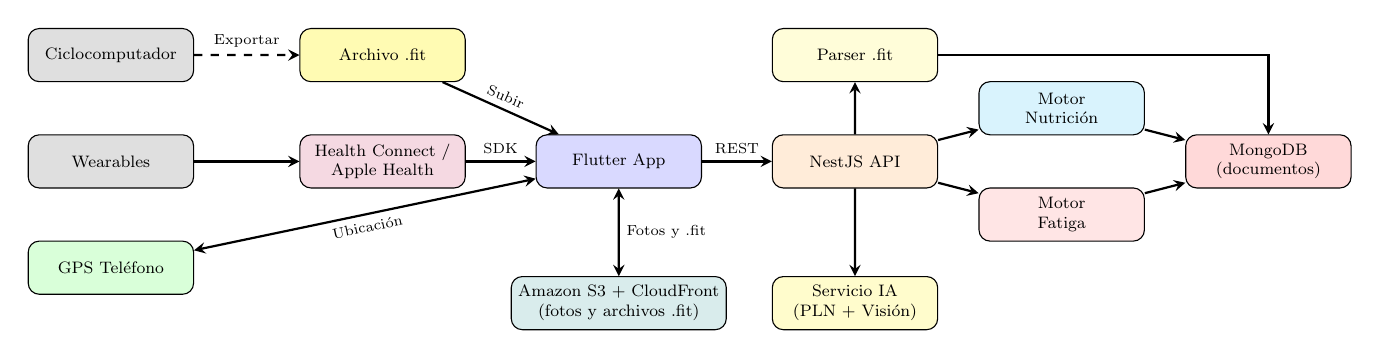
\begin{tikzpicture}[
    box/.style={draw, rectangle, rounded corners, minimum width=2.8cm, minimum height=0.9cm, fill=#1, align=center, font=\footnotesize},
    arrow/.style={->, thick, >=stealth},
    darrow/.style={<->, thick, >=stealth},
    dashed_arrow/.style={->, dashed, thick, >=stealth},
    lbl/.style={font=\scriptsize},
    scale=0.75, transform shape
]
    % Dispositivos del usuario
    \node (ciclo) [box=gray!25] at (-0.6,1.8) {Ciclocomputador};
    \node (wear) [box=gray!25] at (-0.6,0) {Wearables};
    \node (gps) [box=green!15] at (-0.6,-1.8) {GPS Teléfono};

    % Concentradores y archivo exportado
    \node (fit) [box=yellow!30] at (4,1.8) {Archivo .fit};
    \node (hc) [box=purple!15] at (4,0) {Health Connect /\\Apple Health};

    % Aplicación y almacenamiento de archivos
    \node (app) [box=blue!15] at (8,0) {Flutter App};
    \node (s3) [box=teal!15] at (8,-2.4) {Amazon S3 + CloudFront\\(fotos y archivos .fit)};

    % Backend
    \node (api) [box=orange!15] at (12,0) {NestJS API};
    \node (parser) [box=yellow!15] at (12,1.8) {Parser .fit};
    \node (ai) [box=yellow!20] at (12,-2.4) {Servicio IA\\(PLN + Visión)};
    \node (nutri) [box=cyan!15] at (15.5,0.9) {Motor\\Nutrición};
    \node (fatiga) [box=red!10] at (15.5,-0.9) {Motor\\Fatiga};

    % Base de datos
    \node (db) [box=red!15] at (19,0) {MongoDB\\(documentos)};

    % Flechas
    \draw[dashed_arrow] (ciclo) -- node[above, lbl] {Exportar} (fit);
    \draw[arrow] (wear) -- (hc);
    \draw[arrow] (fit) -- node[above, lbl, sloped] {Subir} (app);
    \draw[arrow] (hc) -- node[above, lbl] {SDK} (app);
    \draw[darrow] (gps) -- node[below, lbl, sloped] {Ubicación} (app);
    \draw[darrow] (app) -- node[right, lbl] {Fotos y .fit} (s3);
    \draw[arrow] (app) -- node[above, lbl] {REST} (api);
    \draw[arrow] (api) -- (parser);
    \draw[arrow] (api) -- (ai);
    \draw[arrow] (api) -- (nutri);
    \draw[arrow] (api) -- (fatiga);
    \draw[arrow] (nutri) -- (db);
    \draw[arrow] (fatiga) -- (db);
    \draw[arrow] (parser) -| (db);

\end{tikzpicture}
\captionof{figure}{Arquitectura técnica de la Solución (Alternativa 3).}
\label{fig:arquitectura_solucion}
\end{center}
\newpage
\subsubsection{Módulos Principales y Diagrama de Interacción}
El sistema se divide en módulos funcionales que se comunican entre sí:

\textbf{1. Módulo de Ingesta de Telemetría (El Núcleo de Entrada)}\\
Se encarga de que registrar datos sea lo más simple posible para el deportista, usando tres capas:
\begin{itemize}
    \item Capa Manual: El usuario ingresa sus rutinas (series, repeticiones y peso) o su RPE (percepción subjetiva del esfuerzo).
    \item Capa de Concentradores del SO: La aplicación se sincroniza en segundo plano con Health Connect o Apple Health para obtener datos generales (pasos, calorías activas y frecuencia cardíaca en reposo).
    \item Capa Avanzada (.fit): Para deportistas que usan dispositivos especializados (Garmin, Wahoo, Polar), la API recibe directamente archivos \texttt{.fit}. Un lector (parser) que invoca el backend decodifica el archivo y obtiene datos precisos segundo a segundo (potencia en ciclismo, zonas cardíacas y altimetría).
\end{itemize}

\textbf{2. Motor de Fatiga y Planificación (La Lógica de Negocio Central)}\\
Este módulo cruza los datos fisiológicos que entrega el módulo de ingesta. Al final del día, o después de cada entrenamiento, calcula la carga crónica (CTL) y la carga aguda (ATL). Si el usuario tiene mucha fatiga acumulada por una sesión de resistencia exigente y tiene programada una sesión de fuerza máxima al día siguiente, el sistema le enviará una sugerencia (mediante una notificación push) para que considere bajar el número de series o la carga, y así evitar la interferencia y el sobreentrenamiento. La decisión final queda en manos del usuario.

\textbf{3. Motor de Nutrición Asistida por IA}\\
Deja de lado las metas calóricas fijas y se ajusta según el motor de fatiga. Si el usuario hizo un entrenamiento largo y exigente, el módulo sugiere subir su meta diaria de carbohidratos y la muestra en la aplicación. Además, el usuario puede enviar fotos de sus comidas. NestJS manda la imagen, junto con instrucciones predefinidas (prompt), a la API de visión artificial y recibe una estimación de los macronutrientes. Si la IA tiene poca seguridad en su resultado, le pide al usuario que lo revise, para que los datos guardados sean confiables.
\newpage
\textbf{4. Red Social Deportiva}\\
Este módulo convierte la aplicación en una comunidad. Los usuarios pueden seguir a otras personas, ver un muro con sus publicaciones y publicar en su perfil sus sesiones de fuerza, sus rutas y sus comidas. Lo que lo diferencia es que lo publicado no queda solo como información para leer, sino que se puede usar. Por ejemplo, si un usuario publica su rutina de pecho, otro usuario puede agregarla con un botón a sus rutinas de fuerza, sin copiarla a mano. Lo mismo ocurre con una ruta, que pasa a su módulo de cardio, y con una receta, que pasa a su módulo de nutrición. En el caso de una receta como ``Panqueques Proteicos'', el sistema además ajusta las porciones y los gramos de cada ingrediente para que calcen con lo que ese usuario necesita. Todo lo agregado desde la comunidad entra al cruce de datos como cualquier otro registro. Las fotos de las publicaciones (hasta 4 por publicación) se suben desde el teléfono directamente a Amazon S3 con un permiso temporal que entrega este módulo, y se muestran a través de CloudFront.
\\\\
\textbf{5. Perfil del Usuario y Plan Sugerido}\\
Al registrarse, el usuario responde un cuestionario corto sobre su experiencia, sus objetivos, los días disponibles, su equipamiento, las disciplinas que practica y sus datos corporales básicos. Con eso, el sistema lo clasifica según su nivel (principiante, intermedio o avanzado) y su orientación (más fuerza, más resistencia o equilibrada), y le sugiere un plan semanal a partir de una plantilla para ese perfil. Después, el plan se ajusta con lo que el usuario registra. Si no cumple las sesiones, si reporta un esfuerzo muy alto o si el motor de fatiga detecta una carga excesiva, el sistema sugiere un plan más liviano, y si progresa bien, uno más exigente. El usuario siempre puede modificar o ignorar el plan.
\newpage
El siguiente diagrama muestra cómo se relacionan estos módulos. Las flechas que bajan desde la aplicación indican lo que el usuario envía a cada módulo y lo que recibe de vuelta. Las flechas dentro del backend muestran cómo un módulo usa los resultados de otro. Por ejemplo, la carga de cada sesión alimenta al motor de fatiga, y este ajusta el plan sugerido y las metas de nutrición. Las cajas con borde punteado son servicios externos.

\vspace{0.5cm}
\begin{center}
\setstretch{1}
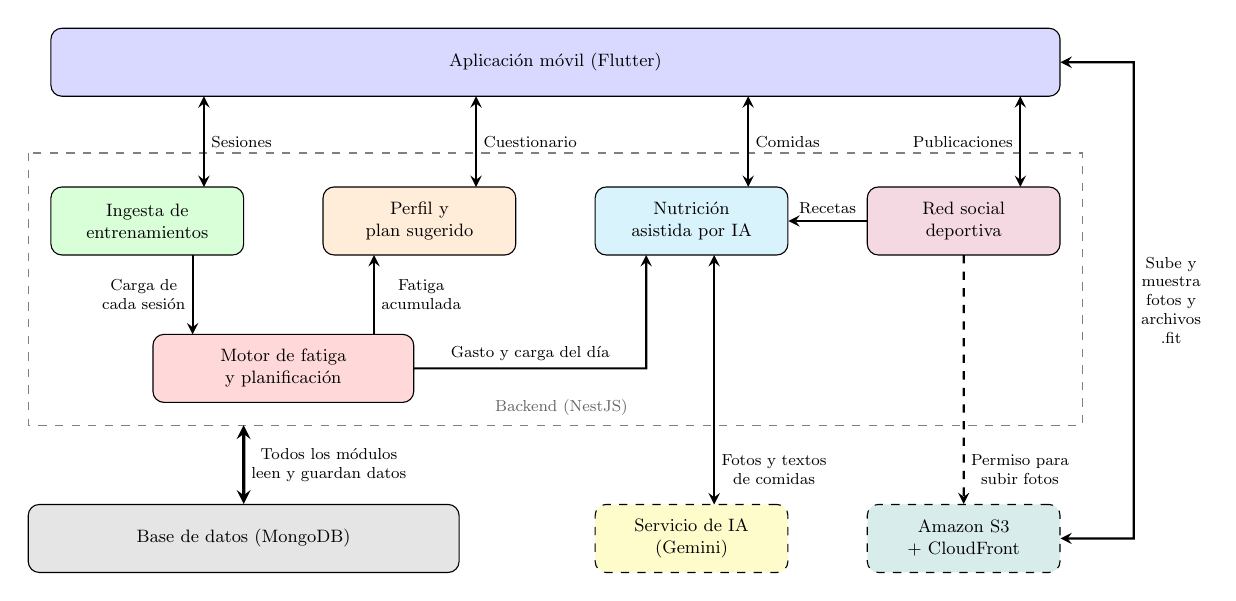
\begin{tikzpicture}[
    box/.style={draw, rectangle, rounded corners, minimum width=3.4cm, minimum height=1.2cm, fill=#1, align=center, font=\small},
    ext/.style={draw, dashed, rectangle, rounded corners, minimum width=3.4cm, minimum height=1.2cm, fill=#1, align=center, font=\small},
    lbl/.style={font=\footnotesize, align=center},
    arrow/.style={->, thick, >=stealth},
    darrow/.style={<->, thick, >=stealth},
    scale=0.72, transform shape
]
    % Aplicación móvil
    \node (ui) [box=blue!15, minimum width=17.8cm] at (7.2,0) {Aplicación móvil (Flutter)};

    % Módulos del backend
    \node (tel) [box=green!15] at (0,-2.8) {Ingesta de\\entrenamientos};
    \node (per) [box=orange!15] at (4.8,-2.8) {Perfil y\\plan sugerido};
    \node (nut) [box=cyan!15] at (9.6,-2.8) {Nutrición\\asistida por IA};
    \node (soc) [box=purple!15] at (14.4,-2.8) {Red social\\deportiva};
    \node (fat) [box=red!15, minimum width=4.6cm] at (2.4,-5.4) {Motor de fatiga\\y planificación};

    % Agrupación del backend
    \draw[dashed, gray] (-2.1,-1.6) rectangle (16.5,-6.4);
    \node[font=\footnotesize, text=gray!80!black, anchor=south east] at (8.6,-6.35) {Backend (NestJS)};

    % Servicios y almacenamiento
    \node (db) [box=gray!20, minimum width=7.6cm] at (1.7,-8.4) {Base de datos (MongoDB)};
    \node (ia) [ext=yellow!20] at (9.6,-8.4) {Servicio de IA\\(Gemini)};
    \node (s3) [ext=teal!15] at (14.4,-8.4) {Amazon S3\\+ CloudFront};

    % Aplicación hacia los módulos
    \draw[darrow] (1.0,-0.6) -- node[lbl, right] {Sesiones} (1.0,-2.2);
    \draw[darrow] (5.8,-0.6) -- node[lbl, right] {Cuestionario} (5.8,-2.2);
    \draw[darrow] (10.6,-0.6) -- node[lbl, right] {Comidas} (10.6,-2.2);
    \draw[darrow] (15.4,-0.6) -- node[lbl, left] {Publicaciones} (15.4,-2.2);

    % Cruces entre módulos
    \draw[arrow] (0.8,-3.4) -- node[lbl, left] {Carga de\\cada sesión} (0.8,-4.8);
    \draw[arrow] (4.0,-4.8) -- node[lbl, right] {Fatiga\\acumulada} (4.0,-3.4);
    \draw[arrow] (fat.east) -- node[lbl, above] {Gasto y carga del día} (8.8,-5.4) -- (8.8,-3.4);
    \draw[arrow] (soc.west) -- node[lbl, above] {Recetas} (nut.east);

    % Hacia servicios externos y datos
    \draw[darrow] (10.0,-3.4) -- node[lbl, right, pos=0.86] {Fotos y textos\\de comidas} (10.0,-7.8);
    \draw[arrow, dashed] (14.4,-3.4) -- node[lbl, right, pos=0.86] {Permiso para\\subir fotos} (s3.north);
    \draw[darrow] (ui.east) -- (17.4,0) -- node[lbl, right] {Sube y\\muestra\\fotos y\\archivos\\.fit} (17.4,-8.4) -- (s3.east);
    \draw[darrow, very thick] (1.7,-6.4) -- node[lbl, right] {Todos los módulos\\leen y guardan datos} (db.north);
\end{tikzpicture}
\captionof{figure}{Diagrama de Interacción entre módulos funcionales.}
\label{fig:interaccion_modulos}
\end{center}
\newpage
\subsubsection{Modelo de Datos (Esquema Conceptual)}
Como los datos del sistema son de tipos muy distintos, la base de datos MongoDB se organizará en colecciones de documentos. Las colecciones principales serán:
\begin{itemize}
    \item \textbf{users (Usuarios):} Guarda las credenciales del usuario y, dentro del mismo documento, su perfil físico, sus metas y los tokens de acceso a servicios de terceros.
    \item \textbf{dailyLogs (Registro Diario):} Un documento por usuario y fecha. Contiene las metas calóricas del día, que se calculan a partir de lo que entrega el motor de fatiga, y los reportes de sensaciones.
    \item \textbf{workouts (Entrenamientos):} Guarda tanto las sesiones de fuerza como las de cardio, diferenciadas por un campo de tipo. En las de fuerza, los ejercicios y las series van dentro del mismo documento.
    \item \textbf{telemetry (Telemetría):} Colección de series temporales que guarda los datos segundo a segundo de potencia y pulsaciones que llegan desde la capa avanzada.
    \item \textbf{posts y follows (Red Social):} Guardan las publicaciones de cada usuario (sesiones, rutas o comidas) y las relaciones entre seguidores. Las fotos de cada publicación no se guardan aquí, solo su dirección en Amazon S3.
    \item \textbf{trainingPlans (Plan Sugerido):} Guarda el plan semanal sugerido de cada usuario, junto con el perfil que se usó para generarlo.
    \item \textbf{meals (Comidas):} Registro de alimentación con sus alimentos dentro del documento. Si se registró con visión artificial, incluye un campo \texttt{aiConfidenceScore} que indica qué tan segura estaba la IA de su estimación.
\end{itemize}
\newpage
\subsubsection{Requerimientos de Infraestructura y Despliegue}
Para ponerla en marcha, la API de NestJS se empaquetará en contenedores \textbf{Docker}. Así, el entorno de desarrollo y el de producción son iguales. La imagen se desplegará en AWS Fargate, el servicio usado en la estimación de costos, que agrega más capacidad automáticamente cuando aumentan las peticiones, por ejemplo cuando muchos usuarios sincronizan sus dispositivos al mismo tiempo.
\\\\
La base de datos se alojará en MongoDB Atlas, el servicio administrado de MongoDB, que hace respaldos automáticos, permite recuperar los datos y cifra el almacenamiento, cumpliendo con los requisitos de ciberseguridad descritos en la factibilidad operativa.
\\\\
Las fotos y los archivos \texttt{.fit} se guardarán en un bucket privado de Amazon S3 en la región de São Paulo, con cifrado activado y una regla que borra los archivos que ya no se usan. Las fotos se mostrarán a través de Amazon CloudFront, que es el único servicio con permiso para leer ese bucket.
\newpage
\subsection{Beneficios del Proyecto}
La plataforma basada en la Alternativa 3 (Solución por Capas) trae varios beneficios, que se pueden separar entre los beneficios para el usuario (el atleta híbrido) y los beneficios comerciales del proyecto.

\textbf{Beneficios para el Usuario (Atleta Híbrido):}
\begin{itemize}
    \item \textbf{Todo en un solo lugar:} El atleta ya no necesita cambiar entre tres aplicaciones distintas (registro de pesas, registro con GPS y contador de calorías). Toda su información deportiva queda en un único panel.
    \item \textbf{Prevención del sobreentrenamiento (fatiga cruzada):} Al cruzar la carga reciente de resistencia con los entrenamientos de fuerza, el sistema avisa al usuario cuando su cuerpo no se ha recuperado y le sugiere bajar las cargas del gimnasio, ayudando a prevenir lesiones y estancamientos.
    \item \textbf{Nutrición ajustada al entrenamiento:} En vez de seguir una meta calórica fija, el atleta recibe sugerencias para tener suficiente glucógeno en los días de resistencia larga y suficiente proteína para recuperar el músculo.
    \item \textbf{Red social con contenido reutilizable:} El usuario puede seguir a otras personas y agregar sus sesiones, rutas y recetas a sus propios módulos con un botón, sin copiar nada a mano. Las recetas se adaptan automáticamente a sus necesidades del día.
    \item \textbf{Plan personalizado:} Incluso sin experiencia previa, el usuario recibe un plan semanal sugerido según su nivel y sus objetivos, que se ajusta con lo que registra.
\end{itemize}
\newpage
\textbf{Beneficios Comerciales y Operativos:}
\begin{itemize}
    \item \textbf{Modelo SaaS escalable:} Como se basa en infraestructura en la nube y en procesamiento automático con IA, el costo de sumar un nuevo suscriptor es muy bajo.
    \item \textbf{Historial acumulado:} A medida que el usuario acumula datos históricos de sus entrenamientos, le resulta menos conveniente cambiarse a otra aplicación o volver al registro manual, lo que favorece que siga usando la plataforma.
    \item \textbf{Ingresos directos:} Los atletas híbridos suelen estar dispuestos a pagar por herramientas que mejoren su rendimiento, lo que facilita conseguir usuarios premium.
\end{itemize}
\newpage
\subsection{Análisis Costo - Beneficio}
El análisis costo-beneficio compara la inversión necesaria para poner en marcha la Solución por Capas con los ingresos y beneficios esperados en un horizonte de 4 años.

\textbf{Estructura de Costos:}
\begin{itemize}
    \item \textbf{Inversión inicial (CAPEX):} Según la factibilidad económica, desarrollar la arquitectura completa (IA, lectura de archivos \texttt{.fit}, backend en NestJS y aplicación en Flutter) requiere una inversión inicial de \$16.230.402 CLP, que corresponde principalmente a horas de desarrollo y a la publicación en las tiendas.
    \item \textbf{Costos operativos anuales (OPEX):} La infraestructura en la nube, el almacenamiento de imágenes, el uso de APIs de IA, el mantenimiento y las licencias se estiman en \$4.543.368 CLP al año, a los que se suman \$601.879 CLP al año de impuesto a la renta. A esto se suman de forma indirecta el Costo de Adquisición de Clientes (CAC) y los gastos de marketing.
\end{itemize}

\textbf{Estructura de Beneficios:}
\begin{itemize}
    \item \textbf{Ingresos recurrentes mensuales (MRR):} La plataforma se financiará con una suscripción premium de \$7.990 CLP al mes.
    \item \textbf{Punto de equilibrio (Break-Even):} Los cálculos financieros mostraron que, para cubrir la inversión inicial y los costos operativos (con un VAN de 0 y una TIR del 15\%), el proyecto necesita mantener en promedio \textbf{159 suscriptores al año} durante 4 años, considerando el IVA, la comisión de las tiendas y el impuesto a la renta.
\end{itemize}

\textbf{Conclusión del Análisis:}\\
La relación costo-beneficio es \textbf{favorable}. Aunque el proyecto requiere un esfuerzo de desarrollo importante y es la alternativa más cara, necesitar 159 suscriptores es poco en comparación con el tamaño del mercado. Reunir en un solo lugar los datos de los dispositivos y las funciones de inteligencia artificial le da a la plataforma una ventaja clara frente a las aplicaciones aisladas, lo que justifica la inversión. Con esto se cierra el análisis de factibilidad y la definición de la arquitectura.

\newpage
